% WBR Perception Implementation -- progress report deck.
% Build: latexmk -xelatex main.tex   (see README.md)
% Content source: docs/SLIDES_OVERVIEW.md, docs/SYSTEM_GUIDE.md, docs/research/.
% Number policy: every number is a DESIGN value, a CALCULATED value, a HOST-TEST
% result, PUBLISHED figure, or explicitly sourced Pi MEASUREMENT; no STM32 measurement.
\documentclass[aspectratio=169,12pt,t]{beamer}

% Speaker notes: uncomment ONE line to see them.
% \setbeameroption{show notes on second screen=right}  % dual-screen (pdfpc)
% \setbeameroption{show only notes}                     % notes handout

\usetheme[progressbar=none, sectionpage=none]{moloch}
% A 208 x 117 mm canvas retains 16:9 and the actual 12pt class fonts.
% Long owner-approved sentences fit without frame scaling or reduced fonts.
\geometry{paperwidth=208mm,paperheight=117mm}

% ---------- fonts ----------
\usepackage{fontspec}
\setsansfont{Avenir Next}[BoldFont={Avenir Next Demi Bold}]
\setmonofont{Menlo}[Scale=1.0]
\newcommand{\captiontype}{\small}

% ---------- palette ----------
\definecolor{navy}{HTML}{1F3A5F}
\definecolor{teal}{HTML}{2A9D8F}
\definecolor{fault}{HTML}{E76F51}
\definecolor{paper}{HTML}{FAFAF7}
\definecolor{ink}{HTML}{22262B}
\definecolor{muted}{HTML}{6B7280}
\definecolor{rule}{HTML}{D6D9DE}

\setbeamercolor{normal text}{fg=ink, bg=paper}
\setbeamercolor{frametitle}{fg=paper, bg=navy}
\setbeamercolor{progress bar}{fg=teal, bg=rule}
\setbeamercolor{alerted text}{fg=fault}
\setbeamercolor{example text}{fg=teal}
\setbeamercolor{structure}{fg=navy}
\setbeamercolor{title separator}{fg=teal}
\setbeamercolor{footline}{fg=muted}
% Beamer otherwise inherits the fault/alert color for in-slide citations.
\setbeamercolor{bibliography entry author}{fg=navy}
\setbeamercolor{bibliography entry title}{fg=ink}
\setbeamercolor{bibliography entry location}{fg=muted}
\setbeamercolor{bibliography entry note}{fg=muted}
\setbeamercolor{block title}{fg=paper, bg=navy}
\setbeamercolor{block body}{bg=navy!6}
\setbeamerfont{frametitle}{size=\large, series=\bfseries}
\setbeamertemplate{frametitle}{\nointerlineskip\begin{beamercolorbox}[wd=\paperwidth,sep=2mm,leftskip=4mm]{frametitle}\usebeamerfont{frametitle}\insertframetitle\strut\end{beamercolorbox}}
\setbeamertemplate{itemize items}{\color{teal}\rule[0.25ex]{0.45em}{0.45em}}
\setbeamertemplate{bibliography item}[text]
\setbeamertemplate{page number in head/foot}[totalframenumber]
\hypersetup{colorlinks=true, linkcolor=navy, urlcolor=navy, citecolor=navy}
% Keep the appendix bookmark free of Beamer translation commands.
\pdfstringdefDisableCommands{\def\translate#1{#1}}

\setbeamertemplate{itemize subitem}{\color{muted}--}

% ---------- packages ----------
\usepackage{tikz}
\usetikzlibrary{arrows.meta, positioning, automata, calc, shapes.geometric, fit, backgrounds, decorations.pathreplacing}
\usepackage{booktabs}
\usepackage{array}
\newcolumntype{L}[1]{>{\raggedright\arraybackslash}p{#1}}
\usepackage{amsmath}
\usepackage{siunitx}
\sisetup{detect-all}

% ---------- helpers ----------
\newcommand{\muted}[1]{{\color{muted}#1}}

% \slideimg[<max height>]{<width>}{<V-id>}{<caption for placeholder>}
% Shows images/<V-id>.jpg or .png if present, otherwise a labelled gray box of the same size.
\newcommand{\slideimg}[4][0.64\textheight]{%
  \IfFileExists{images/#3.jpg}{%
    \includegraphics[width=#2, height=#1, keepaspectratio]{images/#3.jpg}%
  }{\IfFileExists{images/#3.png}{%
    \includegraphics[width=#2, height=#1, keepaspectratio]{images/#3.png}%
  }{%
    \begin{tikzpicture}
      \node[draw=rule, fill=black!6, rounded corners=2pt, minimum width=\dimexpr#2-1pt\relax, outer sep=0pt,
            minimum height=#1, align=center, text width=\dimexpr#2-8mm\relax, font=\small, text=muted]
        {\textbf{#3}\\[2pt]#4\\[2pt]\small Illustration pending};
    \end{tikzpicture}%
  }}%
}

\tikzset{
  box/.style={draw=navy, fill=white, rounded corners=2pt, align=center, font=\small,
              minimum height=7mm, inner sep=3pt},
  flow/.style={-{Stealth[length=2mm]}, thick, color=navy},
  faultflow/.style={-{Stealth[length=2mm]}, thick, color=fault},
  lbl/.style={font=\small, color=ink, fill=paper, inner sep=1pt},
}

% Only the page number appears in the footer.
\setbeamerfont{footline}{size=\small}
\setbeamertemplate{footline}{\hbox{\begin{beamercolorbox}[wd=\paperwidth,ht=4mm,dp=1mm,rightskip=6mm]{footline}\hfill\insertframenumber/\inserttotalframenumber\end{beamercolorbox}}}
\AtBeginSection{\begin{frame}[c]\centering{\Huge\bfseries\color{navy}\thesection. \insertsectionhead\par}\end{frame}}
\setbeamertemplate{navigation symbols}{}
\setbeamersize{text margin left=6mm,text margin right=6mm}
\setlength{\tabcolsep}{4pt}
\renewcommand{\arraystretch}{1.02}
\title{WBR Perception Implementation}
\subtitle{A gate-by-gate engineering guide}
\author{}
\institute{}
\date{13 October 2026}


\newcounter{slidefigure}
\newcommand{\figcap}[1]{\par\smallskip{\centering\captiontype\color{muted}\refstepcounter{slidefigure}Figure \theslidefigure: #1\par}}
\newcommand{\figagain}[1]{\par\smallskip{\centering\captiontype\color{muted}Figure~\ref{fig:#1}: \csuse{caption#1}\par}}
\setbeamerfont{bibliography entry author}{size=\normalsize}
\setbeamerfont{bibliography entry title}{size=\normalsize}
\setbeamerfont{bibliography entry location}{size=\normalsize}
\setbeamerfont{bibliography entry note}{size=\normalsize}
\setlength{\emergencystretch}{2em}
\setbeamerfont{normal text}{size=\normalsize}
\setbeamerfont{itemize/enumerate body}{size=\normalsize}
\setbeamerfont{itemize/enumerate subbody}{size=\normalsize}
\linespread{1.12}
\AtBeginDocument{\setlength{\leftmargini}{1.1em}\setlength{\leftmarginii}{1.2em}\setlength{\labelsep}{.35em}}
\newcommand{\namedcap}[2]{\figcap{#2}}
% Apply spacing after Beamer has created each list (including nested lists).
\usepackage{etoolbox}
\makeatletter
\apptocmd{\itemize}{\ifnum\@itemdepth=1\setlength{\itemsep}{.55em}\else\setlength{\itemsep}{.25em}\fi\setlength{\parsep}{0pt}\setlength{\parskip}{0pt}\setlength{\topsep}{0pt}}{}{}
\makeatother
\newsavebox{\figurebox}
\newcommand{\fig}[3][.48\textheight]{%
  \ifcsdef{diagram#2}{\sbox{\figurebox}{\csuse{diagram#2}}}{%
    \sbox{\figurebox}{\includegraphics[width=\linewidth,height=#1,keepaspectratio]{images/#2.jpg}}}%
  \par\centering\begin{minipage}{\wd\figurebox}\centering
  \usebox{\figurebox}%
  \ifcsdef{assetcaption#2}{\csuse{assetcaption#2}}{%
    \csgdef{assetcaption#2}{\repeatassetcap{#2}}%
    \csgdef{assettext#2}{#3}\figcap{#3}%
    \csxdef{assetnumber#2}{\theslidefigure}}\end{minipage}\par}
\newcommand{\repeatassetcap}[1]{\par\smallskip{\centering\captiontype\color{muted}%
  \begingroup\renewcommand{\label}[1]{}Figure \csuse{assetnumber#1}: \csuse{assettext#1}\par\endgroup}}
\makeatletter
\newcommand{\takeaway}[1]{\global\beamer@framebottomskip=0pt\par\medskip\begin{beamercolorbox}[wd=\linewidth,sep=0pt]{block body}%
  \begin{tabular}{@{}!{\color{teal}\vrule width 3pt}p{\dimexpr\linewidth-22pt\relax}@{}}\normalsize\strut #1\strut\end{tabular}%
  \end{beamercolorbox}\par}
\makeatother


% Course additions retain the approved palette, canvas, type and figure system.
\newcommand{\evidence}[1]{{\small\bfseries\color{teal!70!black}#1}\par\medskip}
\newcommand{\coursefigure}[3]{\begin{minipage}{\linewidth}\centering#2\figcap{\label{fig:#1}#3}\end{minipage}}



\newcommand{\deckitems}[1]{\begin{itemize}#1\end{itemize}}
\newcommand{\deckflow}[1]{\begin{tikzpicture}[node distance=9mm]
\foreach \txt [count=\i] in {#1}{\node[box,font=\normalsize,text width=33mm,minimum height=14mm] (n\i) at ({mod(\i-1,4)*4.7},{-floor((\i-1)/4)*2.4}) {\txt};}
\end{tikzpicture}}

\begin{document}\raggedright
\begin{frame}[c]\relax
{\centering\huge\bfseries\color{navy}WBR Perception Implementation\par}
{\centering\Large\color{teal}A gate-by-gate engineering guide\par}
\medskip{\color{teal}\hrule height .6pt}\vfill
\begin{columns}[T,onlytextwidth]\begin{column}{.48\textwidth}
\large Intel RealSense D435i\par\medskip
Raspberry Pi 5 / ROS 2 Jazzy\par\medskip
ORB-SLAM3 stereo-inertial\par\medskip
STM32H7 controller boundary\par\medskip
\normalsize Figure~\ref{fig:P01} identifies the conceptual platform.
\end{column}\begin{column}{.48\textwidth}
\coursefigure{P01}{\slideimg[.42\textheight]{\linewidth}{P01}{Conceptual perception platform}}{Platform objects; no validation claim.}
\end{column}\end{columns}\vfill
{\centering\color{muted}Engineering and evidence snapshot\quad 13 October 2026\par}
\note{Owner, lecturer and senior audience. No invented identity or affiliation. The owner confirms no Pi gate has passed; restart at N0. Figure is conceptual.}
\end{frame}
\begin{frame}{Contents}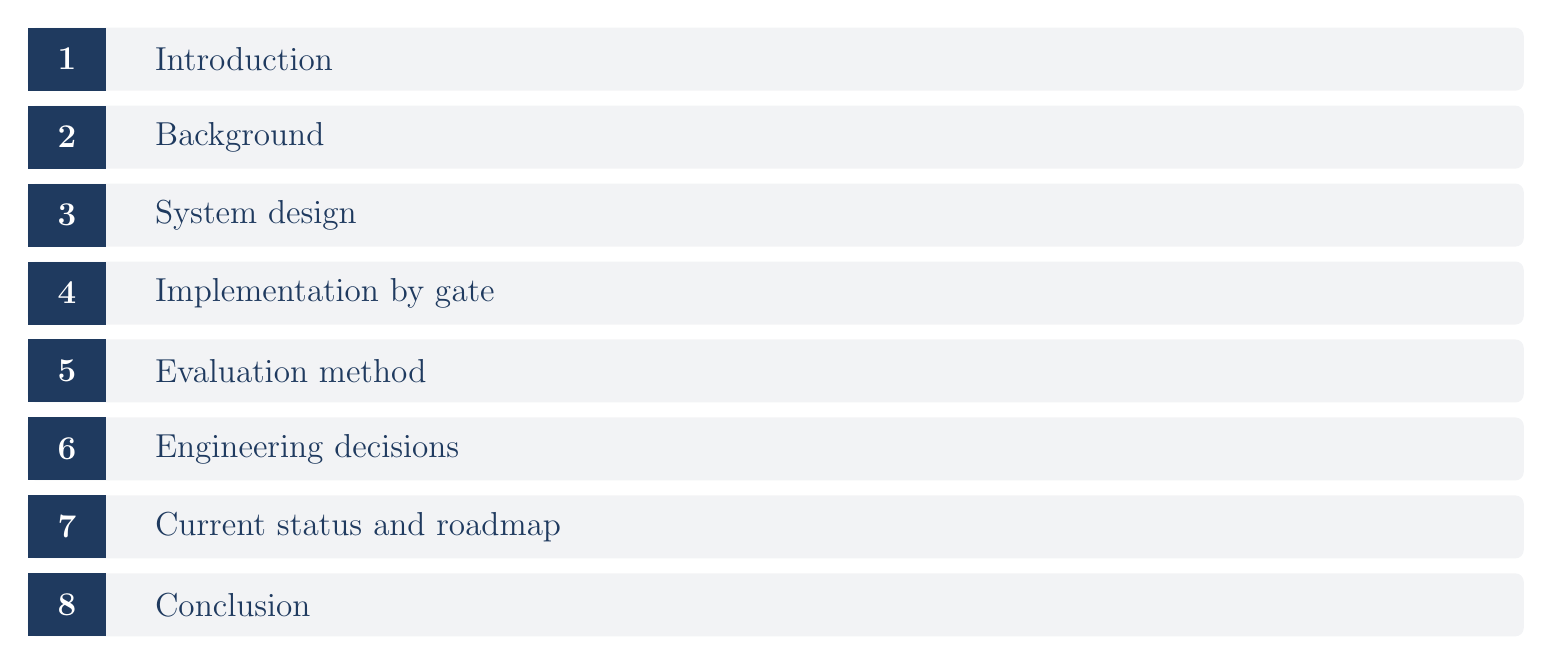
\begin{tikzpicture}
\node[fill=navy!6,rounded corners=3pt,minimum width=190mm,minimum height=8mm,anchor=west] at (0,-0.99) {};
\node[fill=navy,text=white,minimum width=10mm,minimum height=8mm,anchor=west,font=\large\bfseries] at (0,-0.99) {1};
\node[anchor=west,text=navy,font=\large] at (1.5,-0.99) {Introduction};
\node[fill=navy!6,rounded corners=3pt,minimum width=190mm,minimum height=8mm,anchor=west] at (0,-1.98) {};
\node[fill=navy,text=white,minimum width=10mm,minimum height=8mm,anchor=west,font=\large\bfseries] at (0,-1.98) {2};
\node[anchor=west,text=navy,font=\large] at (1.5,-1.98) {Background};
\node[fill=navy!6,rounded corners=3pt,minimum width=190mm,minimum height=8mm,anchor=west] at (0,-2.9699999999999998) {};
\node[fill=navy,text=white,minimum width=10mm,minimum height=8mm,anchor=west,font=\large\bfseries] at (0,-2.9699999999999998) {3};
\node[anchor=west,text=navy,font=\large] at (1.5,-2.9699999999999998) {System design};
\node[fill=navy!6,rounded corners=3pt,minimum width=190mm,minimum height=8mm,anchor=west] at (0,-3.96) {};
\node[fill=navy,text=white,minimum width=10mm,minimum height=8mm,anchor=west,font=\large\bfseries] at (0,-3.96) {4};
\node[anchor=west,text=navy,font=\large] at (1.5,-3.96) {Implementation by gate};
\node[fill=navy!6,rounded corners=3pt,minimum width=190mm,minimum height=8mm,anchor=west] at (0,-4.95) {};
\node[fill=navy,text=white,minimum width=10mm,minimum height=8mm,anchor=west,font=\large\bfseries] at (0,-4.95) {5};
\node[anchor=west,text=navy,font=\large] at (1.5,-4.95) {Evaluation method};
\node[fill=navy!6,rounded corners=3pt,minimum width=190mm,minimum height=8mm,anchor=west] at (0,-5.9399999999999995) {};
\node[fill=navy,text=white,minimum width=10mm,minimum height=8mm,anchor=west,font=\large\bfseries] at (0,-5.9399999999999995) {6};
\node[anchor=west,text=navy,font=\large] at (1.5,-5.9399999999999995) {Engineering decisions};
\node[fill=navy!6,rounded corners=3pt,minimum width=190mm,minimum height=8mm,anchor=west] at (0,-6.93) {};
\node[fill=navy,text=white,minimum width=10mm,minimum height=8mm,anchor=west,font=\large\bfseries] at (0,-6.93) {7};
\node[anchor=west,text=navy,font=\large] at (1.5,-6.93) {Current status and roadmap};
\node[fill=navy!6,rounded corners=3pt,minimum width=190mm,minimum height=8mm,anchor=west] at (0,-7.92) {};
\node[fill=navy,text=white,minimum width=10mm,minimum height=8mm,anchor=west,font=\large\bfseries] at (0,-7.92) {8};
\node[anchor=west,text=navy,font=\large] at (1.5,-7.92) {Conclusion};
\end{tikzpicture}\end{frame}
\begin{frame}{1.1 Robot context}\evidence{KNOWN ownership / PLANNED integration}
\begin{columns}[T,onlytextwidth]\begin{column}{.48\textwidth}\deckitems{\item Wheel-biped robot (WBR) navigation needs useful scene-relative motion. (Figure~\ref{fig:P02})\item STM32H7 keeps body estimation and balance locally.\item Perception adds optional navigation information above that controller.}\end{column}\begin{column}{.48\textwidth}
\coursefigure{P02}{\slideimg[.49\textheight]{\linewidth}{P02}{Navigation context}}{Navigation context; conceptual.}\end{column}\end{columns}
\vfill\takeaway{Qualify perception without making balance depend on Linux.}
\note{The Pi failure requirement is an ownership invariant, not measured physical stability. Actual geometry, mounting and motion budgets remain unknown. Source register: A. Wheel-biped robot (WBR) perception supports navigation while STM32 retains balance.}\end{frame}
\begin{frame}{1.2 Engineering problem}\evidence{PLANNED}
\deckitems{\item A pose may be plausible yet stale or expressed in the wrong frame. (Figure~\ref{fig:D05})\item Timing and calibration errors can survive a successful launch.\item Linux stalls must remove optional autonomy inputs safely.}
\vfill
\coursefigure{D05}{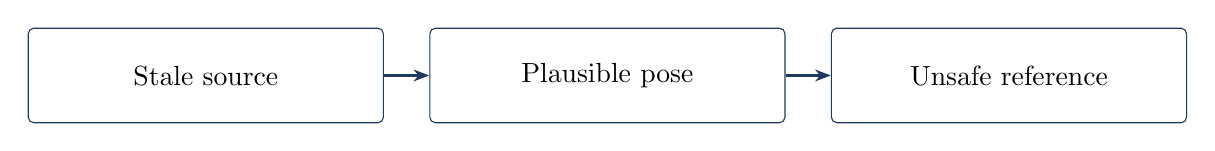
\begin{tikzpicture}[y=.70cm]
\node[box,font=\normalsize,text width=43mm,minimum height=12mm] (a0) at (0.0,0) {Stale source};
\node[box,font=\normalsize,text width=43mm,minimum height=12mm] (a1) at (5.1,0) {Plausible pose};
\draw[flow] (a0.east) -- (a1.west);
\node[box,font=\normalsize,text width=43mm,minimum height=12mm] (a2) at (10.2,0) {Unsafe reference};
\draw[flow] (a1.east) -- (a2.west);\end{tikzpicture}}{Engineering problem; schematic.}
\vfill\takeaway{A valid number is not necessarily a usable estimate.}
\note{Bottom-up qualification separates transport continuity, clock semantics, geometry, algorithm state and receiver policy. No robot safety test has been completed. Source register: A,B. A plausible pose can be stale, misframed or uncalibrated; Linux failure must not remove balance.}\end{frame}
\begin{frame}{1.3 Objectives and research questions}\evidence{PLANNED}
\deckitems{\item Qualify physical input before estimation.\item Reproduce estimation on immutable recorded inputs.\item Measure accuracy, continuity, latency and resource limits.\item Review a health boundary before controller integration.}
\vfill

\par\medskip\textbf{Operational questions}: Sustain exact input? Initialize repeatedly? Reject stale/reset poses? Identify the first resource limit.\par\vfill\takeaway{Each objective needs its own evidence and acceptance review.}
\note{ Source register: B,O. Qualify input, reproduce estimation, quantify quality and define the safe boundary.}\note{Merged original page 7: 
\deckitems{\item Can the Pi sustain the exact input without unexplained gaps?\item Can stereo-inertial estimation initialize and track repeatedly?\item Can a receiver reject stale, invalid or reset estimates?\item Which resource or timing limit fails first?}
\vfill
\begin{block}{Engineering decision}The answer must include failed runs, unknown counters and the limits of each claim.\end{block}
\vfill\takeaway{Fix hypotheses and budgets before collecting comparison runs.}
 Source register: B,O. Can the Pi sustain trusted inputs, initialize repeatedly and supply fresh useful estimates within measured resources?}\end{frame}
\begin{frame}{2.1 Stereo geometry}\evidence{KNOWN method}
\deckitems{\item Infrared (IR) stereo matches one scene point in two views. \hyperlink{referencepage}{[1]}  (Figure~\ref{fig:D09})\item Rectified horizontal disparity d gives depth $Z=fb/d$.\item Intrinsics, baseline b and correspondence determine geometric validity.}
\vfill
\coursefigure{D09}{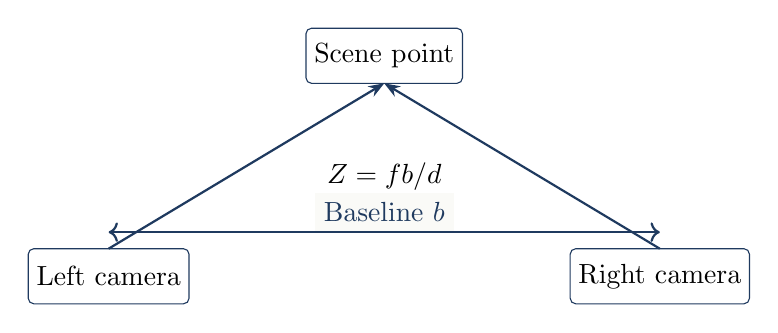
\begin{tikzpicture}[font=\normalsize,y=.70cm]
\coordinate (l) at (0,0);\coordinate (r) at (7,0);\coordinate (p) at (3.5,3);
\node[box,font=\normalsize] at (0,-.5) {Left camera};\node[box,font=\normalsize] at (7,-.5) {Right camera};\node[box,font=\normalsize] at (3.5,3.5) {Scene point};
\draw[flow] (l)--(p);\draw[flow] (r)--(p);\draw[<->,navy,thick] (0,.3)--node[above,fill=paper]{Baseline $b$}(7,.3);
\node at (3.5,1.3) {$Z = f b / d$};\end{tikzpicture}}{Stereo geometry; schematic.}
\vfill\takeaway{Stereo depth requires calibrated geometry and valid image pairing.}
\note{This equation assumes a rectified pinhole pair and nonzero disparity. Here f is focal length in pixels, b is baseline in metres, and Z is metres. No numeric baseline is asserted. See the selected ORB parser and camera profile. Source register: U,RS. Infrared (IR) correspondence and calibrated baseline yield depth; rectification supports reliable pairing.}\end{frame}
\begin{frame}{2.2 Visual-inertial estimation}\evidence{KNOWN method / PLANNED run}
\begin{columns}[T,onlytextwidth]\begin{column}{.48\textwidth}\deckitems{\item Visual-inertial odometry (VIO) combines image constraints and motion. \hyperlink{referencepage}{[1]}  (Figure~\ref{fig:P03})\item An inertial measurement unit (IMU) measures rotation and acceleration.\item Images constrain drift; inertial propagation bridges image intervals.}\end{column}\begin{column}{.48\textwidth}
\coursefigure{P03}{\slideimg[.49\textheight]{\linewidth}{P03}{Visual and inertial motion cues}}{Visual and inertial motion cues; conceptual.}\end{column}\end{columns}
\vfill\takeaway{The camera IMU supports perception, not STM32 balance.}
\note{ORB-SLAM3 tightly integrates visual and inertial constraints. The body controller has an independent IMU, mount, clock and calibration. Do not infer integration from shared names. Source register: P,A. Visual-inertial odometry (VIO) combines images with inertial measurement unit (IMU) motion, distinct from body control.}\end{frame}
\begin{frame}{2.3 Odometry and mapping}\evidence{KNOWN method / PLANNED output}
\deckitems{\item Simultaneous localization and mapping (SLAM) reuses mapped places. \hyperlink{referencepage}{[1]}  (Figure~\ref{fig:D11})\item Loop correction may move the globally consistent map pose.\item Continuous local odometry is a separate output contract.}
\vfill
\coursefigure{D11}{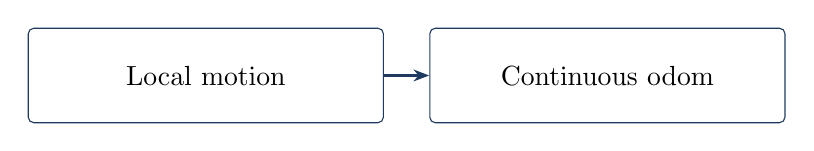
\begin{tikzpicture}[y=.70cm]
\node[box,font=\normalsize,text width=43mm,minimum height=12mm] (a0) at (0.0,0) {Local motion};
\node[box,font=\normalsize,text width=43mm,minimum height=12mm] (a1) at (5.1,0) {Continuous odom};
\draw[flow] (a0.east) -- (a1.west);\end{tikzpicture}\par\medskip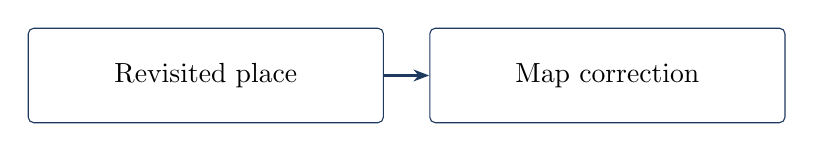
\begin{tikzpicture}[y=.70cm]
\node[box,font=\normalsize,text width=43mm,minimum height=12mm] (a0) at (0.0,0) {Revisited place};
\node[box,font=\normalsize,text width=43mm,minimum height=12mm] (a1) at (5.1,0) {Map correction};
\draw[flow] (a0.east) -- (a1.west);\end{tikzpicture}}{Odometry and mapping; schematic.}
\vfill\takeaway{A jumping map pose cannot simply be relabeled odom.}
\note{A planned ROS integration must choose map correction and continuous odometry ownership explicitly. No continuous odometry bridge is implemented or approved. Source register: P,A. Simultaneous localization and mapping (SLAM) adds revisiting and map correction; continuity is a separate requirement.}\end{frame}
\begin{frame}{2.4 D435i streams}\evidence{MEASURED active identity / calibration OPEN}
\begin{columns}[T,onlytextwidth]\begin{column}{.48\textwidth}\deckitems{\item Stereo-inertial input needs left/right IR images plus raw motion. \hyperlink{referencepage}{[9]}  (Figure~\ref{fig:P04})\item Active device serial: 317422076650; BMI085.\item Descriptor / chip serial: 327743061057; firmware-update ID is separate.}\end{column}\begin{column}{.48\textwidth}
\coursefigure{P04}{\slideimg[.49\textheight]{\linewidth}{P04}{D435i camera package}}{D435i camera package; conceptual.}\end{column}\end{columns}
\vfill\takeaway{Identify the actual unit and preserve its calibration warning.}
\note{Active identity: experiments/2026-10-13-SESSION\_FACTS\_FOR\_SLIDES.md, section B. Enumerated 5000 Mbps is not N1 PASS; firmware 5.17.3.10. Historical note follows: Historical 2026-09-13 metadata: firmware 5.17.3.10; SDK serial 243322073847; ASIC serial and firmware-update ID each 251843061466; USB descriptor separately observed. Preserve: IMU Calibration is not available, default intrinsic and extrinsic will be used. These are archived observations, not current enumeration. Source register: RS,C. Two IR views and motion support stereo-inertial inputs; unit historically reports BMI085 despite older BMI055 descriptions.}\end{frame}
\begin{frame}{2.5 ROS communication}\evidence{KNOWN method / PLANNED pipeline}
\deckitems{\item Robot Operating System 2 (ROS 2) connects topic publishers and subscribers. \hyperlink{referencepage}{[3]}  (Figure~\ref{fig:D13})\item Data Distribution Service (DDS) supplies transport and delivery policies.\item Receipt does not prove source freshness or correct frame semantics.}
\vfill
\coursefigure{D13}{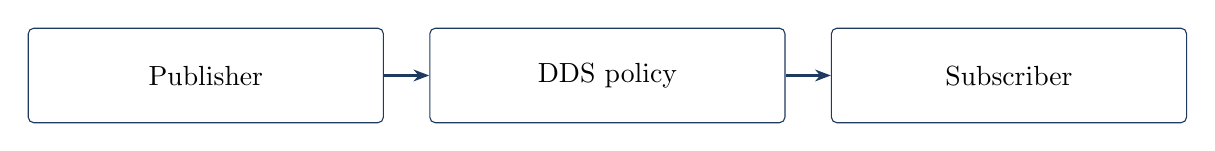
\begin{tikzpicture}[y=.70cm]
\node[box,font=\normalsize,text width=43mm,minimum height=12mm] (a0) at (0.0,0) {Publisher};
\node[box,font=\normalsize,text width=43mm,minimum height=12mm] (a1) at (5.1,0) {DDS policy};
\draw[flow] (a0.east) -- (a1.west);
\node[box,font=\normalsize,text width=43mm,minimum height=12mm] (a2) at (10.2,0) {Subscriber};
\draw[flow] (a1.east) -- (a2.west);\end{tikzpicture}}{ROS communication; schematic.}
\vfill\takeaway{Inspect the graph, policy and data together.}
\note{A node is a graph participant; a process can host several nodes and threads. Message header stamps belong to the producer semantics, not automatically to subscription receipt time. Source register: Q,A. Robot Operating System 2 (ROS 2) topics and Data Distribution Service (DDS) transport do not guarantee usable timely data.}\end{frame}
\begin{frame}{2.6 QoS compatibility}\evidence{KNOWN ROS semantics}
\deckitems{\item Quality of Service (QoS) is an offered/requested contract. \hyperlink{referencepage}{[3]} \item A reliable reader cannot match a best-effort-only writer.\item Sensor observers use best-effort, volatile subscriptions.\item Static transforms use reliable, transient-local delivery.}
\vfill
\begin{tabular}{L{56.666666666666664mm}L{56.666666666666664mm}L{56.666666666666664mm}}\toprule
\textbf{Writer} & \textbf{Reader} & \textbf{Compatible}\\\midrule
Best effort & Reliable & No\\[5pt]
Reliable & Best effort & Yes\\[5pt]
Volatile & Transient local & No\\[5pt]
\bottomrule\end{tabular}
\vfill\takeaway{Topic names alone cannot prove a compatible connection.}
\note{Inspect reliability, durability, history/depth, deadline and lifespan where relevant. Reliable writers can satisfy best-effort readers. A volatile writer cannot satisfy a transient-local reader. Latched context must reach recorder and replay observer. Source register: Q. Quality of Service (QoS) compatibility is offered/requested; reliable subscription cannot consume best-effort-only publication.}\end{frame}
\begin{frame}{3.1 Machine ownership}\evidence{KNOWN ownership}
\deckitems{\item Mac checkout is canonical; preserve its dirty work. (Figure~\ref{fig:D17})\item The Pi acquires and records locally.\item Secure Shell (SSH) carries control and small evidence.\item Use a separate checksummed runtime bundle for each revision.}
\vfill
\coursefigure{D17}{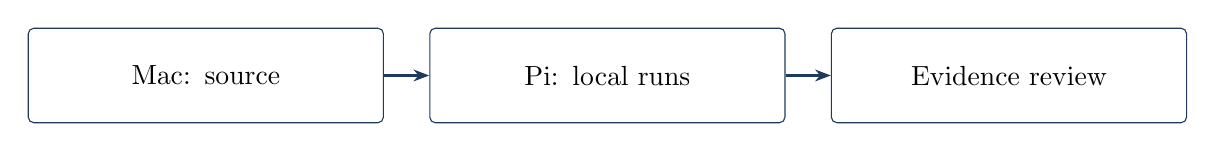
\begin{tikzpicture}[y=.70cm]
\node[box,font=\normalsize,text width=43mm,minimum height=12mm] (a0) at (0.0,0) {Mac: source};
\node[box,font=\normalsize,text width=43mm,minimum height=12mm] (a1) at (5.1,0) {Pi: local runs};
\draw[flow] (a0.east) -- (a1.west);
\node[box,font=\normalsize,text width=43mm,minimum height=12mm] (a2) at (10.2,0) {Evidence review};
\draw[flow] (a1.east) -- (a2.west);\end{tikzpicture}}{Machine ownership; schematic.}
\par\medskip\textbf{Runtime identity}: Hash dirty sources, binaries, libraries and configuration; retain backend, wrapper and launch readback.\par\vfill\takeaway{Deployment copies tools; it does not reset either checkout.}
\note{Installed binaries may differ from checked-out sources. Record source and binary hashes plus exact dependency versions. Large bags stay on independently qualified Pi-local storage. Network configuration changes require approval. Source register: R,N,T. Mac is canonical; Pi acquires locally; Secure Shell (SSH) carries control and small evidence; workstation can supply reference runs.}\note{Merged original page 26: 
\deckitems{\item Record operating system, kernel, packages and compiler identity.\item Hash dirty sources, runtime binaries and configuration.\item Record backend, wrapper, middleware and launch parameters.\item Keep failed runs and original raw logs immutable.}
\vfill
\begin{tabular}{L{87.0mm}L{87.0mm}}\toprule
\textbf{Identity} & \textbf{Retain}\\\midrule
Source & Revision + dirty-file hashes\\[5pt]
Runtime & Binary + library/package versions\\[5pt]
Experiment & Settings + data + command hashes\\[5pt]
\bottomrule\end{tabular}
\vfill\takeaway{A commit identifier alone cannot identify a dirty runtime.}
Historical SDK package 2.58.4 and candidate wrapper 4.58.4 do not imply installed source equivalence. Capture executable and shared-library resolution, vocabulary hash, data hash and run command. Preserve calibration warnings and startup/shutdown logs. Source register: H,T,R. Record packages, source revisions, dirty-file hashes and settings; installed runtime can differ from checkout.}\end{frame}
\begin{frame}{3.2 Control boundary}\evidence{KNOWN ownership / PLANNED validation}
\deckitems{\item Pi: perception, mapping, evaluation and optional autonomy. (Figure~\ref{fig:D18})\item STM32: Linear Quadratic Regulator (LQR) and Virtual Model Control (VMC).\item Its Finite State Machine (FSM), watchdog and motor limits remain local.}
\vfill
\coursefigure{D18}{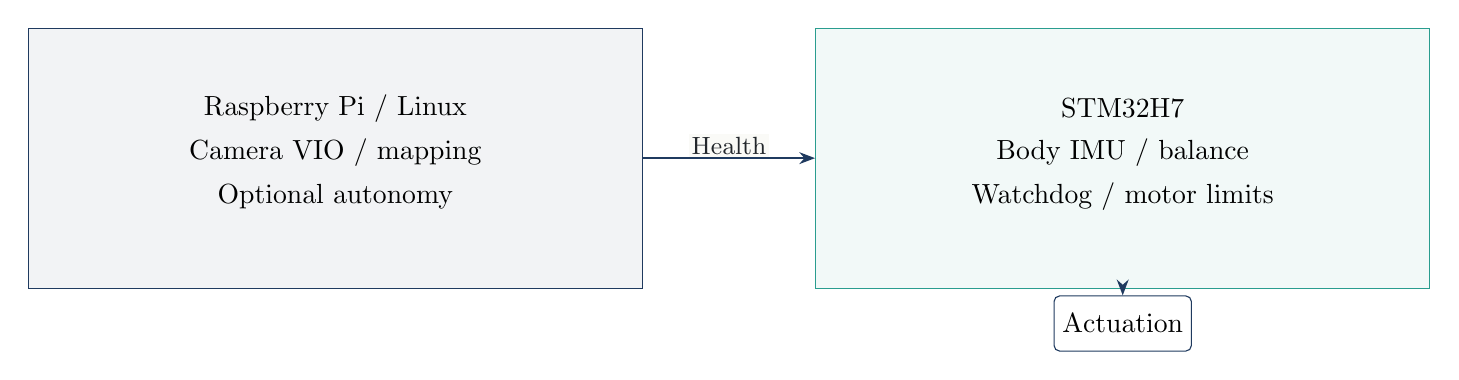
\begin{tikzpicture}[font=\normalsize,y=.70cm]
\node[draw=navy,fill=navy!6,minimum width=78mm,minimum height=33mm] (pi) at (0,0) {};
\node at (0,.9) {Raspberry Pi / Linux};\node at (0,.1) {Camera VIO / mapping};\node at (0,-.7) {Optional autonomy};
\node[draw=teal,fill=teal!6,minimum width=78mm,minimum height=33mm] (mcu) at (10,0) {};
\node at (10,.9) {STM32H7};\node at (10,.1) {Body IMU / balance};\node at (10,-.7) {Watchdog / motor limits};
\draw[flow] (pi.east)--node[above,lbl]{Health}(mcu.west);
\node[box,font=\normalsize] (mot) at (10,-3) {Actuation};\draw[flow] (mcu.south)--(mot);
\end{tikzpicture}}{Control boundary; schematic.}
\vfill\takeaway{Loss of Pi perception must not remove controller ownership.}
\note{LQR, VMC and FSM are controller responsibilities, not implemented in this slide task. The actual transport and command envelope remain planned. Physical balance retention still needs approved staged validation. Source register: A,R. Pi owns perception; STM32H7 owns Linear Quadratic Regulator (LQR), Virtual Model Control (VMC), Finite State Machine (FSM), balance and motor safety.}\end{frame}
\begin{frame}{3.3 Physical platform}\evidence{MEASURED stand-in / PLANNED target}
\begin{columns}[T,onlytextwidth]\begin{column}{.48\textwidth}\deckitems{\item Target: Pi 5 / 8 GB; today: 4 GB / Ubuntu stand-in. \hyperlink{referencepage}{[9]}  (Figure~\ref{fig:P05})\item Target bulk storage: Non-Volatile Memory Express (NVMe); absent today.\item Today boots from 32 GB micro Secure Digital (microSD).}\end{column}\begin{column}{.48\textwidth}
\coursefigure{P05}{\slideimg[.49\textheight]{\linewidth}{P05}{Supply and cooling preparation}}{Supply and cooling preparation; conceptual.}\end{column}\end{columns}
\vfill\takeaway{The target bill of materials is not platform qualification.}
\note{The active-cooler illustration is conceptual. Today: Pi 5 4 GB, 32 GB microSD, 5 V/3 A; source: experiments/2026-10-13-SESSION\_FACTS\_FOR\_SLIDES.md. Historical reports mention different memory inventory and a Raspibase fan. Fresh N0 must record the actual device; do not overwrite history with the target specification. Source register: S,N,PI. Pi 5 8 GB, Ubuntu and Non-Volatile Memory Express (NVMe) storage are the target; actual supply/cooling/storage must be documented anew.}\end{frame}
\begin{frame}{3.4 Sensor-to-pose execution path}\evidence{PLANNED / no gate PASS}
Universal Serial Bus 3 (USB3) feeds the Software Development Kit (SDK).\par\par\medskip\coursefigure{D20}{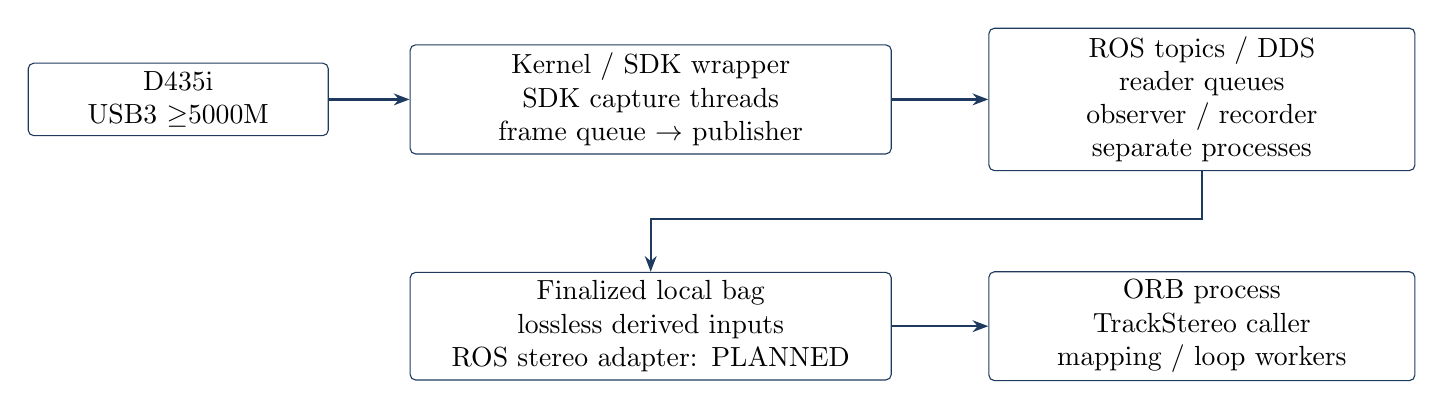
\begin{tikzpicture}[y=.8cm,font=\normalsize,box/.append style={font=\normalsize}]
\node[box,text width=36mm] (sensor) at (0,0) {D435i\\USB3 $\geq$5000M};
\node[box,text width=59mm] (wrapper) at (6,0) {Kernel / SDK wrapper\\SDK capture threads\\frame queue $\to$ publisher};
\node[box,text width=52mm] (dds) at (13,0) {ROS topics / DDS\\reader queues\\observer / recorder\\separate processes};
\draw[flow] (sensor)--(wrapper);
\draw[flow] (wrapper)--(dds);
\node[box,text width=59mm] (bag) at (6,-3.6) {Finalized local bag\\lossless derived inputs\\ROS stereo adapter: PLANNED};
\node[box,text width=52mm] (orb) at (13,-3.6) {ORB process\\TrackStereo caller\\mapping / loop workers};
\draw[flow] (dds.south)--(13,-1.9)--(6,-1.9)--(bag.north);
\draw[flow] (bag)--(orb);
\end{tikzpicture}}{The offline branch isolates estimator behavior from live queues.}\par\medskip IR1/info 15, gyro 200, accel 100 Hz; readers: best effort / volatile.\vfill\takeaway{In Figure~\ref{fig:D20}, N3 is IR1-only; the stereo estimator branch requires a reviewed IR2 extension.}\note{Source: experiments/2026-09-12-pi5-native-sensor-validation/PHASE\_A\_RUNBOOK.md. Commands are teaching examples only; none executed. UNKNOWN budgets require approval.}\end{frame}
\begin{frame}{3.4 Topic and type contract}\evidence{PLANNED / no gate PASS}
\par\begin{tabular}{@{}L{73mm}L{69mm}L{38mm}@{}}\toprule
\textbf{Topic below /camera/camera} & \textbf{Message / cadence} & \textbf{Reader policy}\\\midrule
\texttt{infra1/image\_rect\_raw} & \texttt{sensor\_msgs/msg/Image}; 15 Hz & Best effort / volatile\\[6pt]
\texttt{infra1/camera\_info} & \texttt{sensor\_msgs/msg/CameraInfo}; 15 Hz & Best effort / volatile\\[6pt]
\texttt{gyro/sample}; \texttt{accel/sample} & \texttt{sensor\_msgs/msg/Imu}; 200 / 100 Hz & Best effort / volatile\\[6pt]
\texttt{/tf\_static} (absolute topic) & \texttt{tf2\_msgs/msg/TFMessage}; static & Reliable / transient local\\[6pt]
\bottomrule\end{tabular}\par\vfill\takeaway{Rates are requested baseline values; verify offers, depth and actual delivery.}\note{Source: experiments/2026-09-12-pi5-native-sensor-validation/PHASE\_A\_RUNBOOK.md; n3\_topics.json; ROS Jazzy QoS [3]. Commands are teaching examples only; none executed. UNKNOWN budgets require approval.}\end{frame}
\begin{frame}{3.6 Queues and backpressure}\evidence{PLANNED}
\deckitems{\item A First-In First-Out (FIFO) queue sends its oldest item first. (Figure~\ref{fig:D22})\item Bound each SDK, DDS, executor, recorder and estimator buffer.\item Record arrival/dequeue times, depth and discard policy.\item An unavailable drop counter is UNKNOWN, never zero.}
\vfill
\coursefigure{D22}{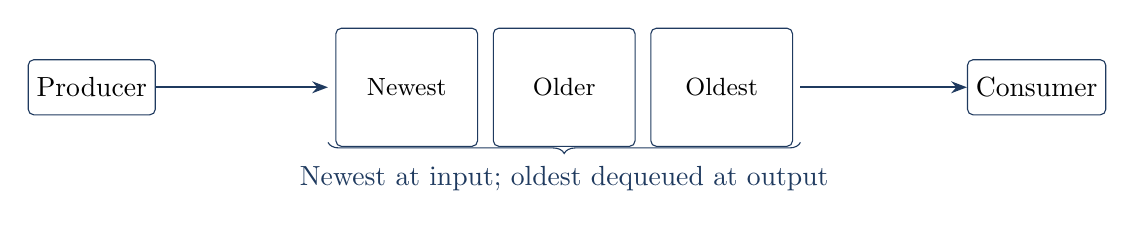
\begin{tikzpicture}[font=\normalsize,y=.70cm]
\node[box,font=\normalsize] (p) at (0,0) {Producer};
\foreach \x/\t in {4/Newest,6/Older,8/Oldest}{\node[box,minimum width=18mm,minimum height=15mm] at (\x,0) {\t};}
\node[box,font=\normalsize] (c) at (12,0) {Consumer};
\draw[flow] (p.east)--(3,0);\draw[flow] (9,0)--(c.west);
\draw[decorate,decoration={brace,mirror,amplitude=4pt},navy] (3,-1)--node[below=5pt]{Newest at input; oldest dequeued at output}(9,-1);
\end{tikzpicture}}{Queues and backpressure; schematic.}
\par\medskip\textbf{Thread ownership}: SDK, wrapper/executor and recorder own separate queues; tracking runs on its caller; mapping/loop workers run separately.\par\vfill\takeaway{A deep queue can preserve delivery while destroying freshness.}
\note{Queue instrumentation is planned. Distinguish producer sequence gaps, observed arrival gaps, recorder count mismatch and measured queue overflow. Latest-only processing may bound age but discards input; inertial coverage must remain consistent. Source register: G,Q,U. Trace SDK/DDS/executor/recorder/estimator queues and policies; unknown drop counters remain UNKNOWN.}\note{Merged original page 22: 
\begin{columns}[T,onlytextwidth]\begin{column}{.48\textwidth}\begin{block}{Acquisition / ROS}SDK callbacks deliver sensor frames. Wrapper work and DDS buffering precede the observer and recorder. Each queue can add age or discard input.\end{block}\end{column}\begin{column}{.48\textwidth}\begin{block}{Estimator / Atlas}\texttt{TrackStereo} runs in its caller. Local mapping consumes keyframes; loop closing handles place recognition and map changes. Atlas is shared map state [1].\end{block}\end{column}\end{columns}\medskip Record queue capacity, depth, arrival/dequeue time and discard policy at each owned boundary; unavailable counters stay UNKNOWN.\vfill\takeaway{A recorder count mismatch and a tracking stall can originate in different queues.}Source: experiments/2026-09-12-pi5-native-sensor-validation/PHASE\_A\_RUNBOOK.md; upstream System.cc. Commands are teaching examples only; none executed. UNKNOWN budgets require approval.}\end{frame}
\begin{frame}{3.8 Storage qualification}\evidence{PLANNED}
\begin{columns}[T,onlytextwidth]\begin{column}{.48\textwidth}\deckitems{\item Pin mount source, partition and Universally Unique Identifier (UUID). (Figure~\ref{fig:P06})\item Measure overall and worst-batch writes, then hashed readback.\item micro Secure Digital (microSD): operating system and small logs.}\end{column}\begin{column}{.48\textwidth}
\coursefigure{P06}{\slideimg[.49\textheight]{\linewidth}{P06}{Separate bulk-data storage}}{Separate bulk-data storage; conceptual.}\end{column}\end{columns}
\par\medskip\textbf{Payload lower bounds}: IR1/15: 4.608 MB/s; stereo/15: 9.216 MB/s. Prepared stereo/30: 18.432 MB/s before overhead; qualify that load separately.\par\vfill\takeaway{Qualify the actual data device before any bag recording.}
\note{Runbook storage proposal: at least 1 GiB and 60 s, overall and worst-batch throughput at least 9.216 decimal MB/s, fsync per 64 MiB batch, SHA-256 readback and finalized cleanup. Default 8 GiB budget may finish too early; a larger write needs review. Retain 10 GiB headroom. No formatting, mounting or storage probe runs here. Source register: G,R. Pin mount source/UUID/device identity and measured throughput/readback; microSD is for operating system and small logs.}\note{Merged original page 24: 
\deckitems{\item Y8 stores one eight-bit grayscale byte per pixel; no compression assumed.\item IR1 payload: 640 $\times$ 480 $\times$ 1 $\times$ 15 = 4.608 MB/s.\item Stereo image payload doubles to 9.216 MB/s before overhead.\item Metadata, motion, serialization and filesystem traffic add load.}
\vfill
\begin{block}{Engineering decision}Qualify sustained recording under real load; theoretical USB speed is not available throughput.\end{block}
\vfill\takeaway{Payload arithmetic is a lower bound, not throughput evidence.}
MB uses decimal 1,000,000 bytes. Y8 is eight-bit grayscale. A 300-second IR1 image-payload equivalent is 1.3824 GB; N2 vendor CSV does not actually store those full image pixels. The storage floor 9.216 MB/s is a margin for IR1, not qualification for stereo recording. Source register: G,U. Calculated IR1 payload is 640$\times$480$\times$1$\times$15 = 4.608 decimal MB/s; stereo doubles image payload before overhead.}\end{frame}
\begin{frame}{3.10 Frame definitions}\evidence{KNOWN conventions / PLANNED mounts}
\deckitems{\item The transform (TF) system relates parent and child frames. \hyperlink{referencepage}{[4]}  (Figure~\ref{fig:D26})\item Body convention: x forward, y left, z up.\item Optical convention: z forward, x right, y down.\item A pose declares origin, axes, units, reference, child and stamp.}
\vfill
\coursefigure{D26}{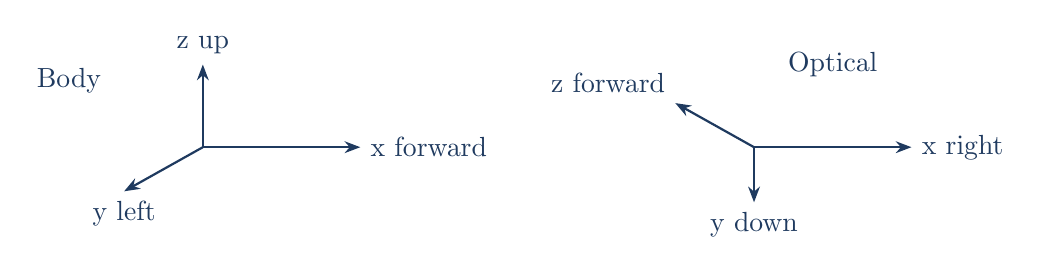
\begin{tikzpicture}[font=\normalsize,y=.70cm]
\node[text=navy] at (-1.7,1.2) {Body};
\draw[flow] (0,0)--(2,0) node[right]{x forward};
\draw[flow] (0,0)--(0,1.5) node[above]{z up};
\draw[flow] (0,0)--(-1,-.8) node[below]{y left};
\node[text=navy] at (8,1.5) {Optical};
\draw[flow] (7,0)--(9,0) node[right]{x right};
\draw[flow] (7,0)--(7,-1) node[below]{y down};
\draw[flow] (7,0)--(6,.8) node[above left]{z forward};
\end{tikzpicture}}{Frame definitions; schematic.}
\vfill\takeaway{Frame names do not define geometry by themselves.}
\note{REP-103 conventions are right-handed. REP-105 map can jump; odom is locally continuous but may drift. world is optional and must be explicitly defined. The estimator body means camera IMU coordinates, not the STM32 robot body. Source register: A,TF. The transform (TF) system relates frames; each pose defines parent/child, axes/origin, units and stamp; world/map/odom differ.}\end{frame}
\begin{frame}{3.11 Robot transform ownership}\evidence{PLANNED / no gate PASS}
\par\medskip\coursefigure{D27}{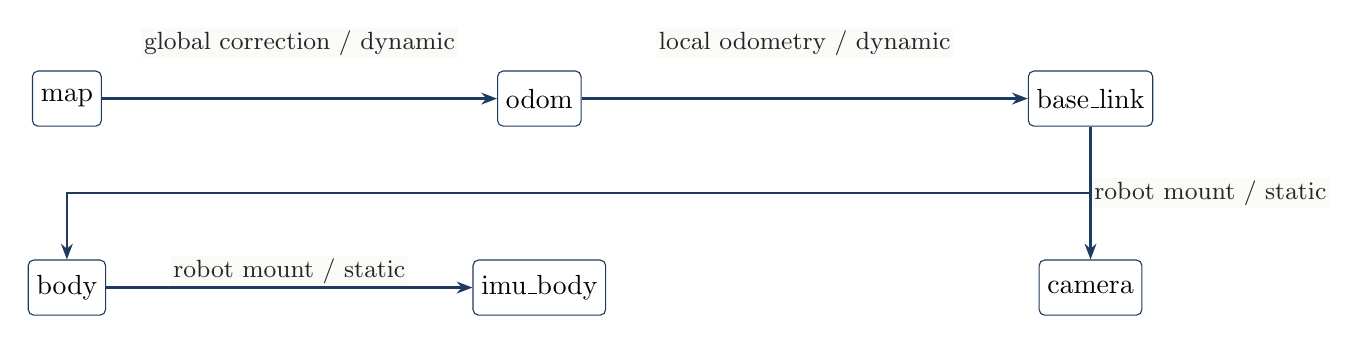
\begin{tikzpicture}[y=.8cm,font=\normalsize,box/.append style={font=\normalsize}]
\node[box] (map) at (0,0) {map};\node[box] (odom) at (6,0) {odom};\node[box] (base) at (13,0) {base\_link};
\draw[flow] (map)--node[above=5mm,lbl]{global correction / dynamic}(odom);
\draw[flow] (odom)--node[above=5mm,lbl]{local odometry / dynamic}(base);
\node[box] (body) at (0,-3) {body};\node[box] (imu) at (6,-3) {imu\_body};\node[box] (cam) at (13,-3) {camera};
\draw[flow] (base.south)--(13,-1.5)--(0,-1.5)--(body.north);
\draw[flow] (body)--node[above,lbl]{robot mount / static}(imu);
\draw[flow] (base)--node[right,lbl]{robot mount / static}(cam);
\end{tikzpicture}}{Dynamic edges need separate planned estimator and continuity owners.}\par\medskip Robot description owns static mounts, including base\_link $\to$ body. The planned bridge owns dynamic edges; implementation is UNKNOWN. Optional world $\to$ map needs an explicit external-reference owner [4].\vfill\takeaway{In Figure~\ref{fig:D27}, one parent and one publisher per child; never relabel a jumping map pose as odom.}\note{Source: docs/ARCHITECTURE.md; REP-103/105. Commands are teaching examples only; none executed. UNKNOWN budgets require approval.}\end{frame}
\begin{frame}{3.12 Camera transform ownership}\evidence{PLANNED / no gate PASS}
\par\medskip\coursefigure{D28}{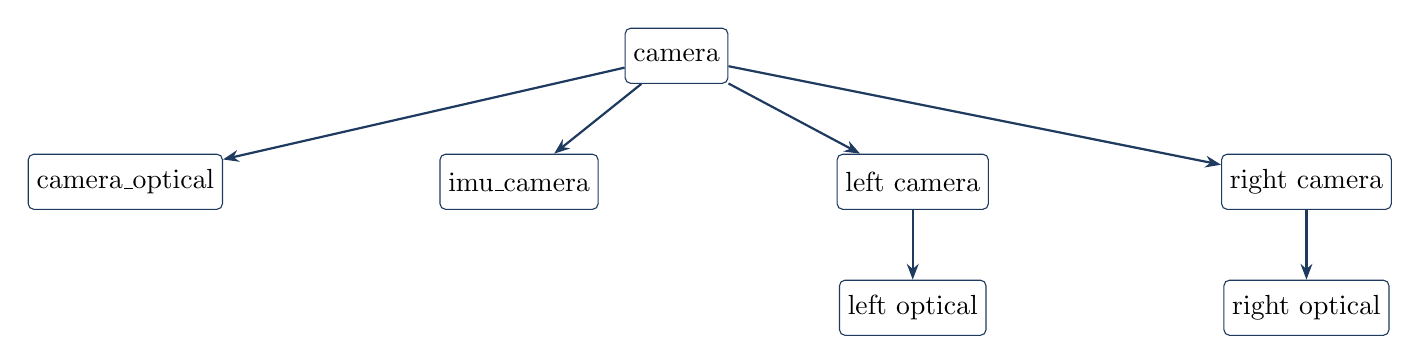
\begin{tikzpicture}[y=.8cm,font=\normalsize,box/.append style={font=\normalsize}]
\node[box] (cam) at (7,0) {camera};
\node[box] (opt) at (0,-2) {camera\_optical};\node[box] (imu) at (5,-2) {imu\_camera};
\node[box] (left) at (10,-2) {left camera};\node[box] (right) at (15,-2) {right camera};
\foreach \n in {opt,imu,left,right}{\draw[flow] (cam)--(\n);}
\node[box] (lo) at (10,-4) {left optical};\node[box] (ro) at (15,-4) {right optical};
\draw[flow] (left)--(lo);\draw[flow] (right)--(ro);
\end{tikzpicture}}{Wrapper-owned sensor geometry is static; frame names here are conceptual.}\par\medskip Wrapper /camera/camera publishes sensor edges on /tf\_static when tf\_publish\_rate=0. Inspect actual parents and frame IDs; do not add this conceptual tree as a second publisher.\vfill\takeaway{In Figure~\ref{fig:D28}, the robot description owns the camera mount; the wrapper owns internal sensor geometry.}\note{Source: experiments/2026-09-12-pi5-native-sensor-validation/PHASE\_A\_RUNBOOK.md; n3\_baseline.yaml. Commands are teaching examples only; none executed. UNKNOWN budgets require approval.}\end{frame}
\begin{frame}{3.13 Independent IMUs}\evidence{KNOWN separation / PLANNED fusion review}
\begin{columns}[T,onlytextwidth]\begin{column}{.48\textwidth}\deckitems{\item Camera IMU: D435i motion for VIO. (Figure~\ref{fig:P07})\item Body IMU: local STM32 balance.\item Mounts, noise and clocks remain separate.\item Fusion needs timing and geometry evidence.}\end{column}\begin{column}{.48\textwidth}
\coursefigure{P07}{\slideimg[.49\textheight]{\linewidth}{P07}{Separate IMU mounting contexts}}{Separate IMU mounting contexts; conceptual.}\end{column}\end{columns}
\vfill\takeaway{Two IMUs are not interchangeable measurements.}
\note{Even nominally equal axes and frequencies do not establish synchronization. Do not substitute camera IMU when Pi fails or feed body IMU to ORB without reviewed calibration and clock mapping. Source register: A,C. D435i IMU supplies VIO; STM32 body IMU supplies balance; no naive fusion across independent clocks/mounts.}\end{frame}
\begin{frame}{3.14 Transform direction}\evidence{KNOWN source convention / PLANNED tests}
\deckitems{\item Camera-to-estimator-IMU transform: $p_b=T_{b\_c1}p_c$. (Figure~\ref{fig:D30})\item Its inverse maps IMU coordinates back into the camera.\item SDK rotation arrays and OpenCV matrix storage orders differ.\item Test basis vectors, inversion and composition.}
\vfill
\coursefigure{D30}{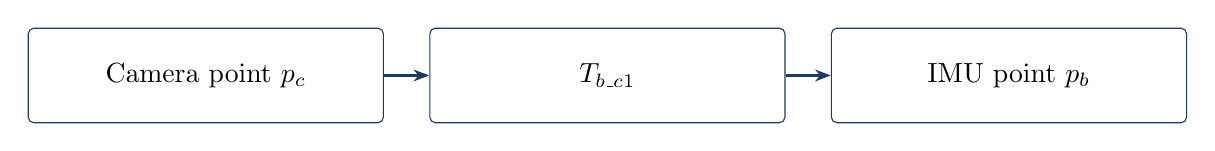
\begin{tikzpicture}[y=.70cm]
\node[box,font=\normalsize,text width=43mm,minimum height=12mm] (a0) at (0.0,0) {Camera point $p_c$};
\node[box,font=\normalsize,text width=43mm,minimum height=12mm] (a1) at (5.1,0) {$T_{b\_c1}$};
\draw[flow] (a0.east) -- (a1.west);
\node[box,font=\normalsize,text width=43mm,minimum height=12mm] (a2) at (10.2,0) {IMU point $p_b$};
\draw[flow] (a1.east) -- (a2.west);\end{tikzpicture}}{Transform direction; schematic.}
\vfill\takeaway{Transform direction must follow code and numeric tests.}
\note{Frame.cc composes T\_cb with T\_bw; ImuTypes.cc stores T\_cb = inverse(T\_bc). SDK rotations are column-major; OpenCV YAML data are row-major. b here denotes estimator IMU/body, never automatically robot body. Identity defaults do not validate a future nonidentity calibration. Source register: C,O,U. p\_b = T\_b\_c1 p\_c; test inverse/basis vectors and column-major SDK versus row-major OpenCV arrays.}\end{frame}
\begin{frame}{3.15 Timestamp fields and domains}\evidence{PLANNED / no gate PASS}
\par\medskip\coursefigure{D31}{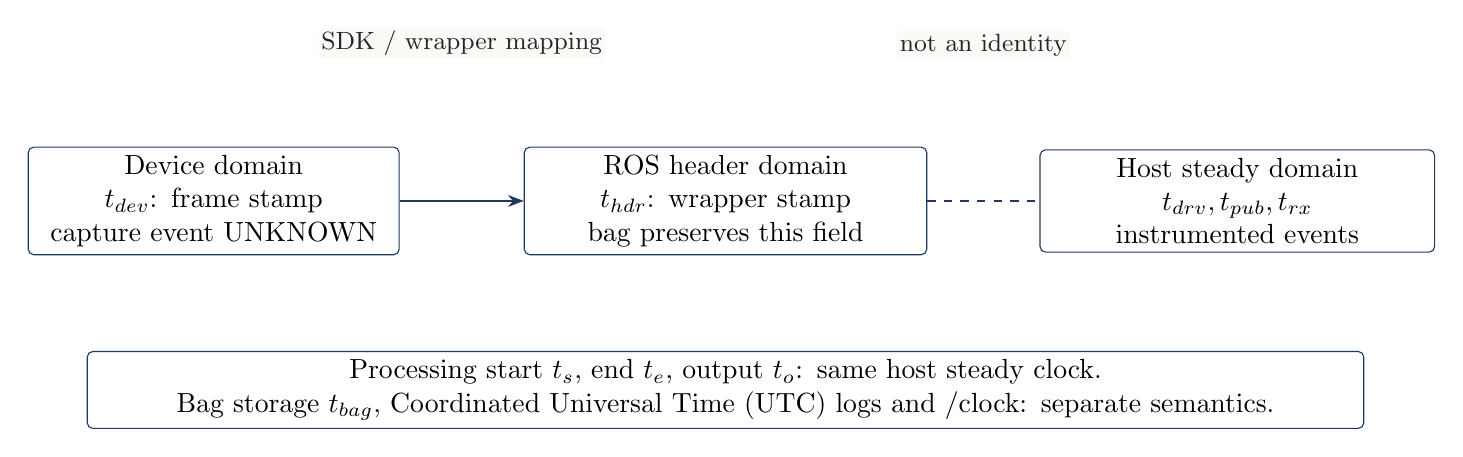
\begin{tikzpicture}[y=.8cm,font=\normalsize,box/.append style={font=\normalsize}]
\node[box,text width=45mm] (dev) at (0,0) {Device domain\\$t_{dev}$: frame stamp\\capture event UNKNOWN};
\node[box,text width=49mm] (ros) at (6.5,0) {ROS header domain\\$t_{hdr}$: wrapper stamp\\bag preserves this field};
\node[box,text width=48mm] (host) at (13,0) {Host steady domain\\$t_{drv},t_{pub},t_{rx}$\\instrumented events};
\draw[flow] (dev)--node[above=18mm,lbl]{SDK / wrapper mapping}(ros);
\draw[dashed,navy] (ros)--node[above=18mm,lbl]{not an identity}(host);
\node[box,text width=160mm] at (6.5,-3) {Processing start $t_s$, end $t_e$, output $t_o$: same host steady clock.\\Bag storage $t_{bag}$, Coordinated Universal Time (UTC) logs and /clock: separate semantics.};
\end{tikzpicture}}{Header epoch, receipt and output are different events even if units match.}\par\medskip Capture $t_c$ is a physical event; exposure convention and device relation are UNKNOWN. Preserve raw stamps and mapping version before defining source age.\vfill\takeaway{In Figure~\ref{fig:D31}, global-time enablement is configuration evidence, not measured synchronization.}\note{Source: experiments/2026-09-12-pi5-native-sensor-validation/PHASE\_A\_RUNBOOK.md; librealsense v2.58.4 global timestamp reader. Commands are teaching examples only; none executed. UNKNOWN budgets require approval.}\end{frame}
\begin{frame}{3.16 Where timestamps are stamped}\evidence{PLANNED / no gate PASS}
\par\begin{tabular}{@{}L{43mm}L{55mm}L{82mm}@{}}\toprule
\textbf{Field / event} & \textbf{Stamp owner} & \textbf{Interpretation}\\\midrule
$t_{dev}$ / sensor frame & Device + SDK metadata & Hardware-relative or mapped domain; inspect each frame\\[6pt]
$t_{hdr}$ / message header & ROS wrapper & Producer epoch; not publish time\\[6pt]
$t_{rx},t_s,t_e,t_o$ & Observer / adapter instrumentation & Local steady-clock receipt, start, end, emission\\[6pt]
$t_{bag}$ / storage record & rosbag2 / storage backend & Recorder time; never substitute for source header\\[6pt]
\bottomrule\end{tabular}\par\vfill\takeaway{A trajectory stamp is the estimated pose epoch, not when its file was written.}\note{Source: experiments/2026-09-12-pi5-native-sensor-validation/PHASE\_A\_RUNBOOK.md; n3\_metrics.py. Commands are teaching examples only; none executed. UNKNOWN budgets require approval.}\end{frame}
\begin{frame}{3.17 Global time}\evidence{PLANNED}
\deckitems{\item Global-time option readback is a configuration observation. \hyperlink{referencepage}{[5]} \item The SDK maps device time toward host time.\item Enabled global time does not measure camera–IMU offset.\item Arrival minus mapped stamp is not pure USB latency.}
\vfill
\begin{tabular}{L{87.0mm}L{87.0mm}}\toprule
\textbf{Observation} & \textbf{What it establishes}\\\midrule
Option enabled & Requested timestamp behavior\\[5pt]
Frame domain & Per-frame clock classification\\[5pt]
Mapped timestamp & Relationship with mapping uncertainty\\[5pt]
Camera–IMU offset & Separate physical alignment measurement\\[5pt]
\bottomrule\end{tabular}
\vfill\takeaway{Record domains and uncertainty before reporting source age.}
\note{Pinned v2.58.4 global\_timestamp\_reader.cpp provides algorithm evidence. Historical metadata read global time 1, but actual frame domains were not measured in that session. Off/on diagnostics must use separate labeled runs and preserve raw stamps. Source register: C,CLK. Enabled global-time option is not measured camera–IMU offset or pure USB latency.}\end{frame}
\begin{frame}{3.18 Worked latency decomposition}\evidence{PLANNED / no gate PASS}
\par\medskip\coursefigure{D34}{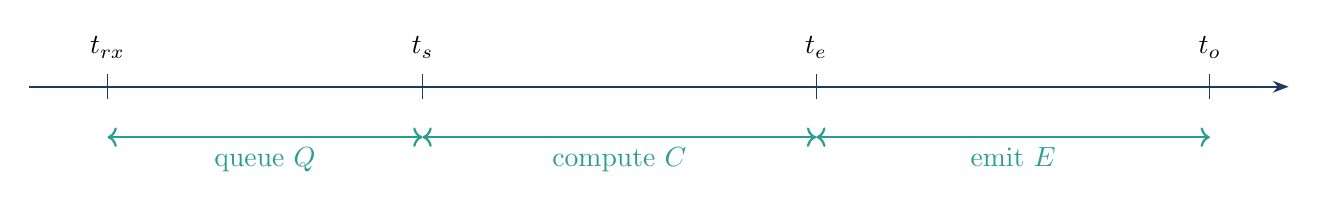
\begin{tikzpicture}[y=.8cm,font=\normalsize,box/.append style={font=\normalsize}]
\draw[flow] (0,0)--(16,0);
\foreach \x/\t in {1/$t_{rx}$,5/$t_s$,10/$t_e$,15/$t_o$}{\draw[navy] (\x,-.2)--(\x,.2);\node[above] at (\x,.3){\t};}
\draw[<->,teal,thick] (1,-.8)--node[below]{queue $Q$}(5,-.8);
\draw[<->,teal,thick] (5,-.8)--node[below]{compute $C$}(10,-.8);
\draw[<->,teal,thick] (10,-.8)--node[below]{emit $E$}(15,-.8);
\end{tikzpicture}}{All three components use the same host steady clock.}\par\medskip $L_{rx\to o}=(t_s-t_{rx})+(t_e-t_s)+(t_o-t_e)=Q+C+E$.\par\medskip Capture age requires $\widehat t_c=g(t_{dev})$ in this domain. If mapping error is bounded by $u$, true age lies in $[t_o-\widehat t_c-u,\ t_o-\widehat t_c+u]$.\vfill\takeaway{In Figure~\ref{fig:D34}, fast compute does not imply fresh output when queue wait dominates.}\note{Source: experiments/2026-09-12-pi5-native-sensor-validation/PHASE\_A\_RUNBOOK.md. Commands are teaching examples only; none executed. UNKNOWN budgets require approval.}\end{frame}
\begin{frame}{3.19 Calibration register}\evidence{NOMINAL active geometry / calibration OPEN}
\deckitems{\item Stereo intrinsics/extrinsics belong to the selected image profiles.\item Camera–IMU extrinsics and time offset need independent validation.\item Candidate noise/walk values are ASSUMED; time offset UNKNOWN.\item SDK computer-aided design (CAD) fallback is not a unit measurement.}
\vfill
\begin{tabular}{L{87.0mm}L{87.0mm}}\toprule
\textbf{Quantity} & \textbf{Current classification}\\\midrule
Image projection & MEASURED active factory readback\\[5pt]
IMU geometry & NOMINAL active factory transform\\[5pt]
IMU noise / offset & ASSUMED noise; offset UNKNOWN\\[5pt]
Stereo readiness & PLANNED separate qualification\\[5pt]
\bottomrule\end{tabular}
\vfill\takeaway{Separate transport acceptance from calibration readiness.}
\note{Current candidate: experiments/2026-10-13-n4b-d435i-prep/D435i\_317422076650\_stereo\_inertial.yaml: nominal factory geometry; noise assumed, not accepted. Preserve verbatim: IMU Calibration is not available, default intrinsic and extrinsic will be used. Historical logs establish CAD fallback, identity sensitivity, zero bias and placeholder zero noise arrays. Do not infer the precise device-side cause from this warning alone. Source register: C. Stereo geometry, camera–IMU extrinsics/time offset and device noise need independent provenance; SDK defaults are not measurements.}\end{frame}
\begin{frame}{3.20 Stereo calibration}\evidence{PLANNED}
\deckitems{\item Match model, resolution, distortion and rectification path. \hyperlink{referencepage}{[6]}  (Figure~\ref{fig:D36})\item Use left/right calibration for the actual paired streams.\item Inspect epipolar vertical residuals and temporal pairing.\item Reject mismatched profiles before feature tuning.}
\vfill
\coursefigure{D36}{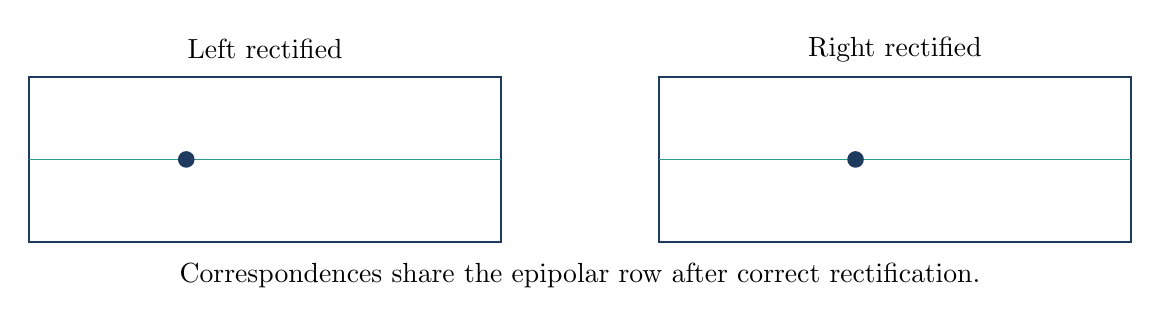
\begin{tikzpicture}[font=\normalsize,y=.70cm]
\foreach \x/\t in {0/Left rectified,8/Right rectified}{\draw[navy,thick] (\x,0) rectangle ++(6,3);\node at (\x+3,3.5){\t};\draw[teal] (\x,1.5)--++(6,0);}
\fill[navy] (2,1.5) circle (3pt);\fill[navy] (10.5,1.5) circle (3pt);
\node at (7,-.6) {Correspondences share the epipolar row after correct rectification.};\end{tikzpicture}}{Stereo calibration; schematic.}
\vfill\takeaway{Wrong geometry can mimic an algorithm failure.}
\note{For rectified images corresponding points should lie on the same horizontal epipolar line. Report residual distributions, target coverage, rejected pairs and timestamp differences; budgets require approval. Do not rectify twice or copy EuRoC calibration into D435i settings. Source register: U,K,C. Match chosen profiles/distortion/rectification; inspect epipolar residuals and left/right time pairing before stereo estimation.}\end{frame}
\begin{frame}{3.21 Calibration capture}\evidence{PLANNED}
\begin{columns}[T,onlytextwidth]\begin{column}{.48\textwidth}\deckitems{\item Measure the fixed target and configuration. \hyperlink{referencepage}{[6]}  (Figure~\ref{fig:P08})\item Excite every axis without blur or saturation.\item Check detections and shared time coverage.\item Capture stationary full-precision noise data.}\end{column}\begin{column}{.48\textwidth}
\coursefigure{P08}{\slideimg[.49\textheight]{\linewidth}{P08}{Target-based calibration preparation}}{Target-based calibration preparation; conceptual.}\end{column}\end{columns}
\vfill\takeaway{A textured-room trajectory is not automatically calibration data.}
\note{Kalibr candidate: measured AprilGrid, safe cable slack, varied viewpoints and excitation. Preserve unsuccessful takes. Follow the readiness procedure only after camera authorization and prerequisite gates. No calibration write or guided capture is performed here. Source register: C,K. PLANNED measured AprilGrid and all-axis motion support calibration; textured-room VIO motion has a different purpose.}\end{frame}
\begin{frame}{3.22 IMU noise}\evidence{PLANNED}
\deckitems{\item Allan deviation compares noise across averaging time $\tau$. \hyperlink{referencepage}{[7]}  (Figure~\ref{fig:D38})\item Short-time slope helps estimate white-noise density.\item Longer records are needed to constrain bias instability or walk.\item Vendor comma-separated values (CSV) round motion; use full precision.}
\vfill
\coursefigure{D38}{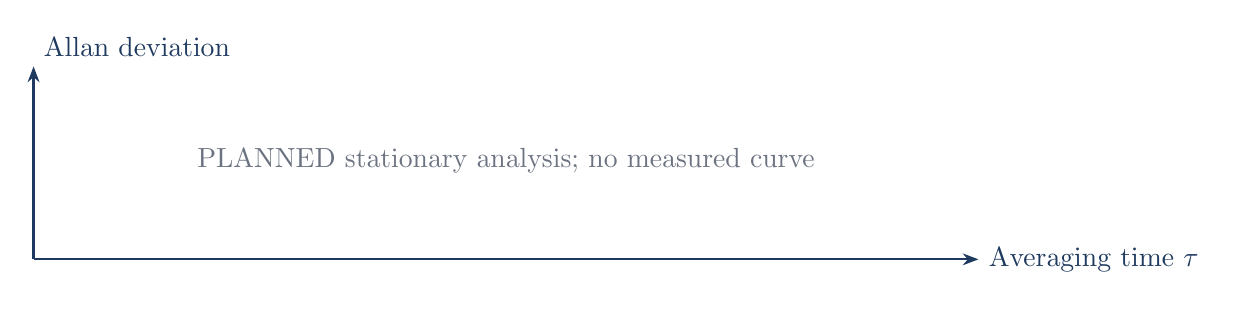
\begin{tikzpicture}[font=\normalsize,y=.70cm]
\draw[flow] (0,0)--(12,0) node[right]{Averaging time $\tau$};\draw[flow] (0,0)--(0,3.5) node[above right]{Allan deviation};
\node[text=muted] at (6,1.8) {PLANNED stationary analysis; no measured curve};\end{tikzpicture}}{IMU noise; schematic.}
\vfill\takeaway{Choose stationary duration from the averaging times you need.}
\note{Allan variance is half the mean squared difference between adjacent interval averages; Allan deviation is its square root. Record sample units/rates, temperature, stationary validity and confidence/sample support. Do not confuse bias instability with random walk. Tool compatibility and unit-specific parameters remain unknown. Source register: C,I. Allan variance/deviation separates noise and bias across averaging times; long enough full-precision stationary input is required.}\end{frame}
\begin{frame}{3.24 Algorithm threads}\evidence{KNOWN algorithm / PLANNED operation}
\deckitems{\item Oriented FAST and Rotated BRIEF (ORB) features link image views. \hyperlink{referencepage}{[1]}  (Figure~\ref{fig:D40})\item FAST: Features from Accelerated Segment Test; BRIEF: Binary Robust Independent Elementary Features.\item Tracking runs on caller; mapping and loop workers optimize.\item Atlas owns multiple maps and merging state.}
\vfill
\coursefigure{D40}{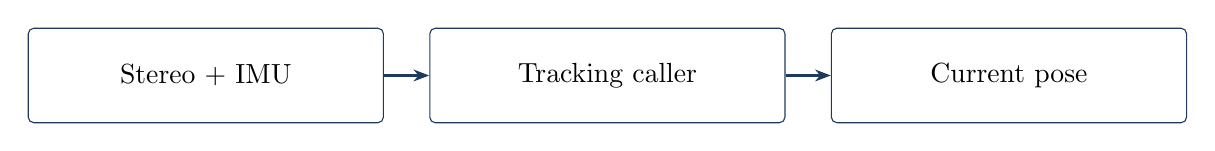
\begin{tikzpicture}[y=.70cm]
\node[box,font=\normalsize,text width=43mm,minimum height=12mm] (a0) at (0.0,0) {Stereo + IMU};
\node[box,font=\normalsize,text width=43mm,minimum height=12mm] (a1) at (5.1,0) {Tracking caller};
\draw[flow] (a0.east) -- (a1.west);
\node[box,font=\normalsize,text width=43mm,minimum height=12mm] (a2) at (10.2,0) {Current pose};
\draw[flow] (a1.east) -- (a2.west);\end{tikzpicture}\par\medskip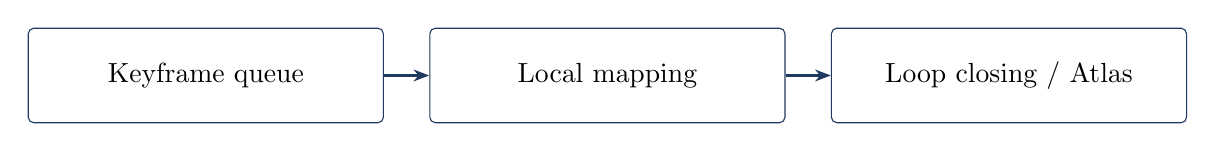
\begin{tikzpicture}[y=.70cm]
\node[box,font=\normalsize,text width=43mm,minimum height=12mm] (a0) at (0.0,0) {Keyframe queue};
\node[box,font=\normalsize,text width=43mm,minimum height=12mm] (a1) at (5.1,0) {Local mapping};
\draw[flow] (a0.east) -- (a1.west);
\node[box,font=\normalsize,text width=43mm,minimum height=12mm] (a2) at (10.2,0) {Loop closing / Atlas};
\draw[flow] (a1.east) -- (a2.west);\end{tikzpicture}}{Algorithm threads; schematic.}
\vfill\takeaway{Thread activity is not equivalent to valid tracking.}
\note{FAST means Features from Accelerated Segment Test; BRIEF means Binary Robust Independent Elementary Features. These expansions belong to the feature components. System.cc starts worker threads; tracking and map corrections need explicit event records. The viewer is additional work, not a prerequisite for a scientifically valid display-free output path. Source register: P,U. ORB-SLAM3 uses Oriented FAST and Rotated BRIEF features (expand component names in notes); tracking/mapping/loop closing have distinct roles.}\end{frame}
\begin{frame}{3.25 Tracking}\evidence{PLANNED}
\deckitems{\item Pair calibrated stereo images at a defined image epoch. \hyperlink{referencepage}{[1]}  (Figure~\ref{fig:D41})\item Attach all required IMU samples over each image interval.\item Extract features, match stereo and predict/optimize pose.\item Inspect tracking state, relocalization and reset before tuning.}
\vfill
\coursefigure{D41}{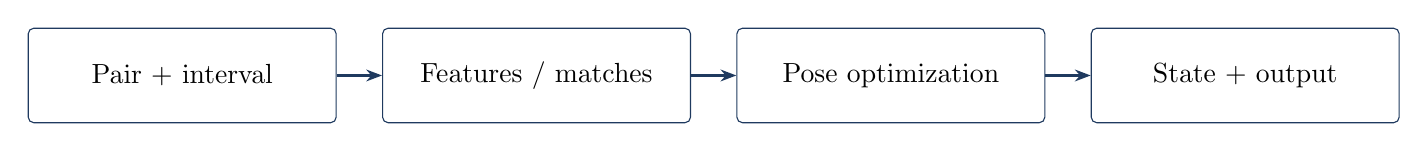
\begin{tikzpicture}[y=.70cm]
\node[box,font=\normalsize,text width=37.0mm,minimum height=12mm] (a0) at (0.0,0) {Pair + interval};
\node[box,font=\normalsize,text width=37.0mm,minimum height=12mm] (a1) at (4.5,0) {Features / matches};
\draw[flow] (a0.east) -- (a1.west);
\node[box,font=\normalsize,text width=37.0mm,minimum height=12mm] (a2) at (9.0,0) {Pose optimization};
\draw[flow] (a1.east) -- (a2.west);
\node[box,font=\normalsize,text width=37.0mm,minimum height=12mm] (a3) at (13.5,0) {State + output};
\draw[flow] (a2.east) -- (a3.west);\end{tikzpicture}}{Tracking; schematic.}
\vfill\takeaway{Every processed image needs accounted motion coverage.}
\note{TrackStereo accepts images, timestamp and vector of IMU measurements. Adapter boundaries need leading and trailing coverage; do not assume example readers guard every boundary. Motion gaps, clock offset, frame error and weak texture require separate diagnosis. Source register: U. Pair stereo images and image-bounded IMU intervals; extract/match features and estimate pose; inspect tracking/reset state before tuning.}\end{frame}
\begin{frame}{3.26 Mapping and Atlas}\evidence{PLANNED}
\deckitems{\item Keyframes retain selected poses and visual constraints. \hyperlink{referencepage}{[1]}  (Figure~\ref{fig:D42})\item Local mapping optimizes nearby structure and inertial state.\item Atlas can create multiple maps and later merge them.\item Loop correction can change the reference transform.}
\vfill
\coursefigure{D42}{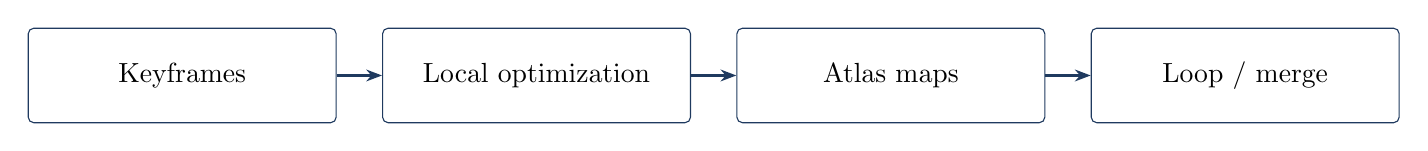
\begin{tikzpicture}[y=.70cm]
\node[box,font=\normalsize,text width=37.0mm,minimum height=12mm] (a0) at (0.0,0) {Keyframes};
\node[box,font=\normalsize,text width=37.0mm,minimum height=12mm] (a1) at (4.5,0) {Local optimization};
\draw[flow] (a0.east) -- (a1.west);
\node[box,font=\normalsize,text width=37.0mm,minimum height=12mm] (a2) at (9.0,0) {Atlas maps};
\draw[flow] (a1.east) -- (a2.west);
\node[box,font=\normalsize,text width=37.0mm,minimum height=12mm] (a3) at (13.5,0) {Loop / merge};
\draw[flow] (a2.east) -- (a3.west);\end{tikzpicture}}{Mapping and Atlas; schematic.}
\vfill\takeaway{Invalidate or re-establish downstream state after map changes.}
\note{A keyframe trajectory is not an all-frame trajectory. Compare coverage separately. Mapping load and loop/global optimization can create resource spikes. Preserve map/session/reset identity in the proposed health contract. Source register: P,U. Local optimization estimates map/inertial state; Atlas manages multiple maps/merging; correction can jump the output frame.}\end{frame}
\begin{frame}{3.27 Inertial initialization}\evidence{PLANNED}
\deckitems{\item Stereo provides metric geometry when calibration is valid. \hyperlink{referencepage}{[1]}  (Figure~\ref{fig:D43})\item Inertial initialization estimates gravity, velocity and biases.\item Sufficient excitation and correct timing remain necessary.\item Record every attempted initialization and reset.}
\vfill
\coursefigure{D43}{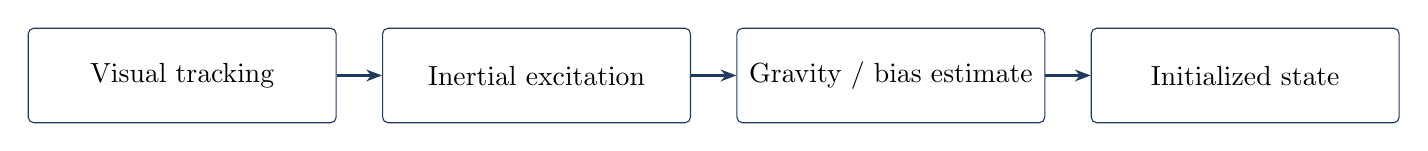
\begin{tikzpicture}[y=.70cm]
\node[box,font=\normalsize,text width=37.0mm,minimum height=12mm] (a0) at (0.0,0) {Visual tracking};
\node[box,font=\normalsize,text width=37.0mm,minimum height=12mm] (a1) at (4.5,0) {Inertial excitation};
\draw[flow] (a0.east) -- (a1.west);
\node[box,font=\normalsize,text width=37.0mm,minimum height=12mm] (a2) at (9.0,0) {Gravity / bias estimate};
\draw[flow] (a1.east) -- (a2.west);
\node[box,font=\normalsize,text width=37.0mm,minimum height=12mm] (a3) at (13.5,0) {Initialized state};
\draw[flow] (a2.east) -- (a3.west);\end{tikzpicture}}{Inertial initialization; schematic.}
\vfill\takeaway{Stereo scale does not remove inertial initialization requirements.}
\note{Avoid transferring monocular unknown-scale wording to stereo. Degenerate motion, wrong noise, sign errors and gaps can defeat initialization despite available depth. Initialization criteria and numerical budgets remain planned. Source register: P,U. Estimate gravity, velocity and biases with sufficient excitation; stereo scale does not remove calibration/timing requirements.}\end{frame}
\begin{frame}{3.28 Settings audit before tuning}\evidence{PLANNED / no gate PASS}
\par\begin{tabular}{@{}L{48mm}L{85mm}L{47mm}@{}}\toprule
\textbf{Pinned parser group} & \textbf{Meaning / check} & \textbf{Failure implication}\\\midrule
Camera1 / Camera2; Stereo & Projection, distortion, b or T\_c1\_c2; selected rectification path & Wrong disparity geometry; scale / epipolar error\\[6pt]
IMU.T\_b\_c1 & Camera $\to$ estimator IMU; numeric basis-vector / inverse test & Axis/sign error; gravity or bias inconsistency\\[6pt]
IMU.Frequency; four noise fields & Continuous-time densities / walks; discretize once & False confidence; unstable initialization\\[6pt]
ORBextractor fields & Feature count, pyramid, FAST thresholds & Tune only after input, timing and calibration\\[6pt]
\bottomrule\end{tabular}\par\vfill\takeaway{The active stereo candidate uses nominal geometry and assumed noise; qualification remains OPEN.}\note{Source: docs/ORB\_SLAM3\_OFFLINE\_PREPARATION.md; upstream pinned stereo\_inertial\_euroc.cc. Commands are teaching examples only; none executed. UNKNOWN budgets require approval.}\end{frame}
\begin{frame}{3.28 Numeric IMU settings contract}\evidence{PLANNED / no gate PASS}
YAML (YAML Ain’t Markup Language) settings must follow the selected pinned parser. All four unit-specific noise quantities remain UNKNOWN.\par\begin{tabular}{@{}L{73mm}L{111mm}@{}}\toprule
\textbf{Key family} & \textbf{Interpretation}\\\midrule
IMU.NoiseGyro / NoiseAcc & Continuous-time gyro / accel noise densities; code multiplies by $\sqrt{f}$\\[6pt]
IMU.GyroWalk / AccWalk & Bias random-walk quantities; code divides by $\sqrt{f}$\\[6pt]
IMU.Frequency / T\_b\_c1 & Input-grid frequency $f$ / camera-to-IMU transform; not raw accel rate\\[6pt]
\bottomrule\end{tabular}\par\medskip Camera.width/height/fps and Camera1/Camera2 keys must match actual inputs. Example EuRoC values describe that dataset; they are not D435i calibration.\vfill\takeaway{Do not discretize densities twice or replace unresolved noise with example values.}\note{Source: docs/ORB\_SLAM3\_OFFLINE\_PREPARATION.md; upstream pinned stereo\_inertial\_euroc.cc. Commands are teaching examples only; none executed. UNKNOWN budgets require approval.}\end{frame}
\begin{frame}{3.29 Input association}\evidence{MEASURED helper/build / camera behavior OPEN}
\deckitems{\item Prepared helper interpolates accel only between valid brackets. (Figure~\ref{fig:D45})\item Use gyro epochs for a reviewed combined input grid.\item Reject gaps, duplicate/backward time and extrapolation.\item Retain originals and every interpolation/rejection decision.}
\vfill
\coursefigure{D45}{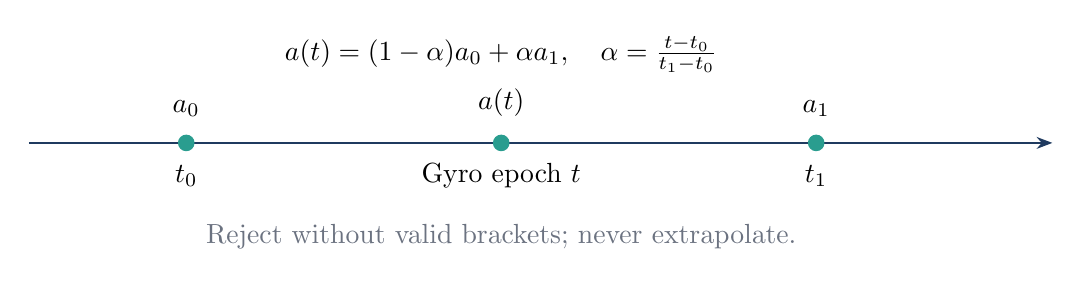
\begin{tikzpicture}[font=\normalsize,y=.70cm]
\draw[flow] (0,0)--(13,0);\foreach \x in {2,6,10}{\fill[teal] (\x,0) circle (3pt);}\node[above] at (2,.3){$a_0$};\node[above] at (6,.3){$a(t)$};\node[above] at (10,.3){$a_1$};
\node at (2,-.6){$t_0$};\node at (6,-.6){Gyro epoch $t$};\node at (10,-.6){$t_1$};
\node at (6,1.6){$a(t)=(1-\alpha)a_0+\alpha a_1,\quad \alpha=\frac{t-t_0}{t_1-t_0}$};
\node[text=muted] at (6,-1.7){Reject without valid brackets; never extrapolate.};\end{tikzpicture}}{Input association; schematic.}
\vfill\takeaway{A 200 Hz input grid does not make raw accel 200 Hz.}
\note{Current helper source: experiments/2026-10-13-n4b-d435i-prep/d435i\_input.h and verification.md (offline/synthetic); Pi build status: experiments/2026-10-13-SESSION\_FACTS\_FOR\_SLIDES.md, section E. No camera behavior measured. a(t) = (1−$\alpha$)a0 + $\alpha$a1 with $\alpha$=(t−t0)/(t1−t0), t0$\leq$t$\leq$t1. Verify known linear signals, irregular spacing, missing endpoints and exact nanosecond conversions. Apply measured time offset once with a tested sign. A candidate mono adapter is not an implemented stereo input path. Source register: O,C. PLANNED accel interpolation on gyro times requires bracketing/gap rejection/no extrapolation; 200 Hz combined input is not 200 Hz raw accel.}\end{frame}
\begin{frame}{3.30 Planned health envelope}\evidence{PLANNED / no gate PASS}
\par\begin{tabular}{@{}L{59mm}L{77mm}L{44mm}@{}}\toprule
\textbf{Field family} & \textbf{Receiver purpose} & \textbf{Current design state}\\\midrule
Version, session, sequence & Reject unknown format, duplicates and old boot & PLANNED; no wire message\\[6pt]
Source epoch, domain, age bound & Distinguish new heartbeat from new estimate & Clock relationship UNKNOWN\\[6pt]
Frames, reset/map ID, state & Reject wrong reference, map jump or initialization & PLANNED semantics\\[6pt]
Pose / velocity / uncertainty & Use only valid finite supported quantities & Covariance availability UNKNOWN\\[6pt]
\bottomrule\end{tabular}\par\par\medskip\textbf{Open choices}: Rate follows useful cadence; transport needs link/load evidence. Age bounds need clock mapping and receiver review; uncertainty needs estimator support.\par\vfill\takeaway{Publication rate, link transport and stale threshold remain UNKNOWN.}\note{Source: docs/ARCHITECTURE.md; docs/DECISIONS.md. Commands are teaching examples only; none executed. UNKNOWN budgets require approval.}\note{Merged original page 103: 
\deckitems{\item Candidate rate follows useful output cadence and receiver capacity.\item Transport choice needs error, bandwidth and timing measurements.\item Stale thresholds require measured age and safety-policy review.\item Uncertainty fields are optional only when justified.}
\vfill
\begin{tabular}{L{87.0mm}L{87.0mm}}\toprule
\textbf{Open choice} & \textbf{Evidence needed before design}\\\midrule
Rate / transport & Useful cadence, load and link errors\\[5pt]
Age threshold & Clock relation and receiver safety policy\\[5pt]
Uncertainty & Estimator-supported interpretation\\[5pt]
\bottomrule\end{tabular}
\vfill\takeaway{Approve the interface before writing messages or firmware.}
Pi and STM32 clocks are independent. Link receipt cannot prove capture freshness without a source-age bound. No fixed transport, Hz, stale timeout or covariance is invented; first-party public API/message changes require approval. Source register: A,R,B. PLANNED rate, transport, thresholds and uncertainty fields await receiver evidence and architecture review.}\end{frame}
\begin{frame}{3.31 Health supervision}\evidence{PLANNED}
\deckitems{\item ABSENT and INITIALIZING are not fresh estimates. (Figure~\ref{fig:D47})\item FRESH requires valid fields, frame/session and bounded source age.\item STALE or INVALID removes optional perception input.\item Reset requires explicit frame/session re-establishment.}
\vfill
\coursefigure{D47}{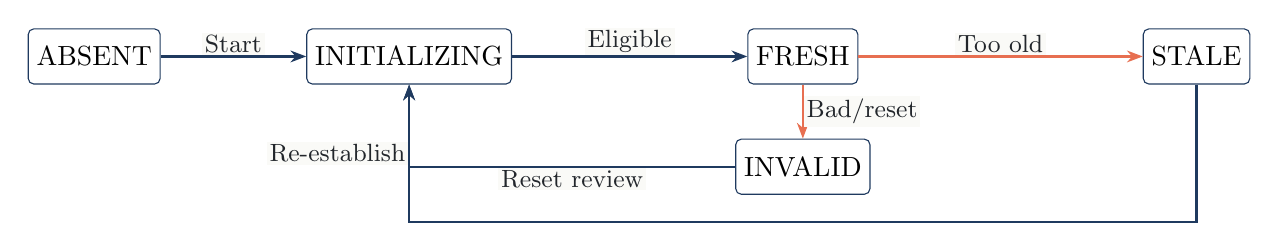
\begin{tikzpicture}[font=\normalsize,y=.70cm]
\node[box,font=\normalsize] (a) at (0,0){ABSENT};\node[box,font=\normalsize] (i) at (4,0){INITIALIZING};\node[box,font=\normalsize] (f) at (9,0){FRESH};\node[box,font=\normalsize] (s) at (14,0){STALE};\node[box,font=\normalsize] (v) at (9,-2){INVALID};
\draw[flow] (a)--node[above,lbl]{Start}(i);\draw[flow] (i)--node[above,lbl]{Eligible}(f);\draw[faultflow] (f)--node[above,lbl]{Too old}(s);\draw[faultflow] (f)--node[right,lbl]{Bad/reset}(v);
\draw[flow] (v.west) -- node[below,lbl]{Reset review} (4,-2) -- (i.south);\draw[flow] (s.south) -- (14,-3) -- (4,-3) -- node[left,lbl]{Re-establish} (i.south);
\end{tikzpicture}}{Health supervision; schematic.}
\vfill\takeaway{A live heartbeat can still accompany stale perception.}
\note{This is a planned semantic state model, not firmware. Wrong frame, nonfinite fields, duplicate sequence, old session and unannounced map jump must reject. Receiver clock wrap, mapping uncertainty and restart behavior need reviewed fixtures. Source register: A,B. PLANNED absent/initializing/fresh/stale/invalid transitions require receiver checks; heartbeat does not prove source freshness.}\end{frame}
\begin{frame}{3.32 Planned Pi-to-STM32 boundary}\evidence{PLANNED / no gate PASS}
\par\medskip\coursefigure{D48}{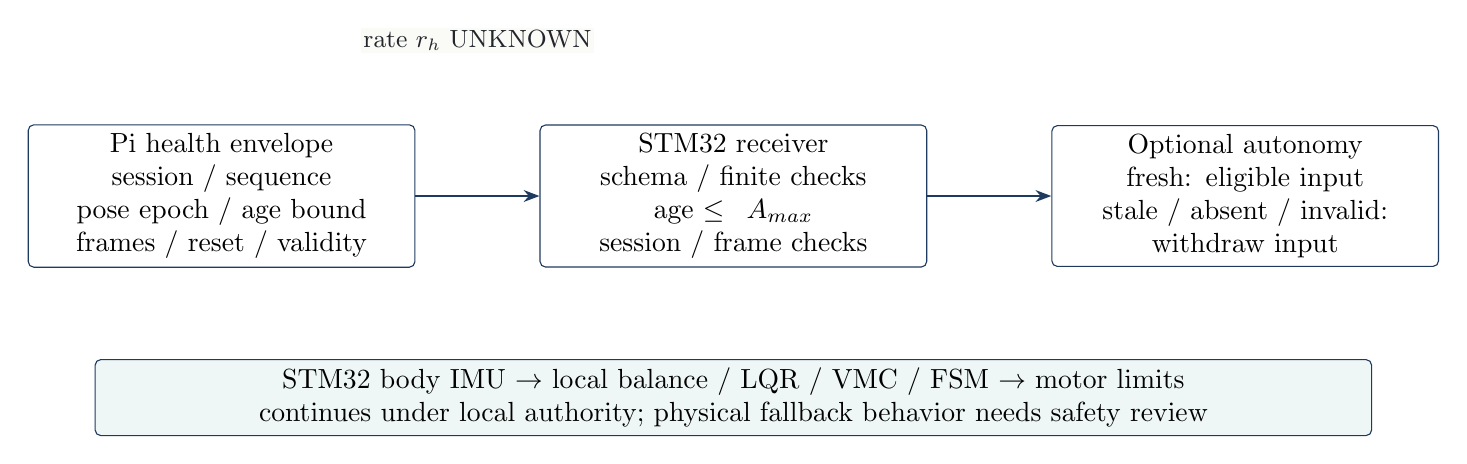
\begin{tikzpicture}[y=.8cm,font=\normalsize,box/.append style={font=\normalsize}]
\node[box,text width=47mm] (pi) at (0,0) {Pi health envelope\\session / sequence\\pose epoch / age bound\\frames / reset / validity};
\node[box,text width=47mm] (rx) at (6.5,0) {STM32 receiver\\schema / finite checks\\age $\leq A_{max}$\\session / frame checks};
\node[box,text width=47mm] (nav) at (13,0) {Optional autonomy\\fresh: eligible input\\stale / absent / invalid:\\withdraw input};
\draw[flow] (pi)--node[above=18mm,lbl]{rate $r_h$ UNKNOWN}(rx);
\draw[flow] (rx)--(nav);
\node[box,text width=160mm,fill=teal!8] at (6.5,-3.2) {STM32 body IMU $\to$ local balance / LQR / VMC / FSM $\to$ motor limits\\continues under local authority; physical fallback behavior needs safety review};
\end{tikzpicture}}{The health path provides optional information; local control keeps authority.}\par\medskip $A_{max}$, transport and $r_h$ require approval. Receiver age must include source age and link residence with a defined clock relation; receipt-only timeout is insufficient.\vfill\takeaway{In Figure~\ref{fig:D48}, these are planned semantics; no message, firmware or stability test is implemented.}\note{Source: docs/ARCHITECTURE.md; docs/DECISIONS.md. Commands are teaching examples only; none executed. UNKNOWN budgets require approval.}\end{frame}
\begin{frame}{4.1 Gate dependencies and status}\evidence{PLANNED / no gate PASS}
\par\medskip\coursefigure{D50}{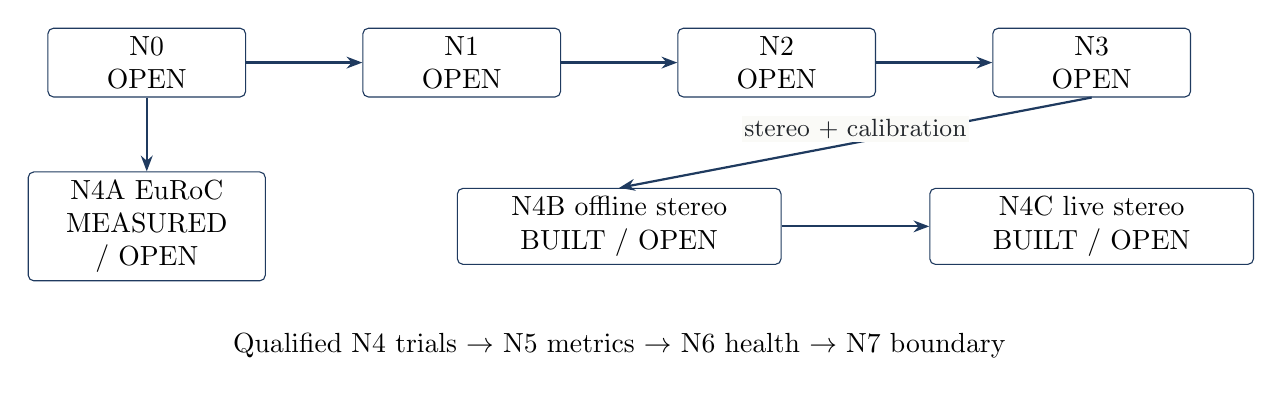
\begin{tikzpicture}[y=.8cm,font=\normalsize,box/.append style={font=\normalsize}]
\foreach \x/\n/\t in {0/a/N0,4/b/N1,8/c/N2,12/d/N3}{\node[box,text width=23mm] (\n) at (\x,0) {\t\\OPEN};}
\draw[flow] (a)--(b);\draw[flow] (b)--(c);\draw[flow] (c)--(d);
\node[box,text width=28mm] (e) at (0,-2.6) {N4A EuRoC\\MEASURED / OPEN};
\node[box,text width=39mm] (f) at (6,-2.6) {N4B offline stereo\\BUILT / OPEN};
\node[box,text width=39mm] (g) at (12,-2.6) {N4C live stereo\\BUILT / OPEN};
\draw[flow] (a)--(e);\draw[flow] (d.south)--node[above,lbl]{stereo + calibration}(f.north);
\draw[flow] (f)--(g);
\node at (6,-4.5) {Qualified N4 trials $\to$ N5 metrics $\to$ N6 health $\to$ N7 boundary};
\end{tikzpicture}}{N4A is independent of camera gates; N4B requires N3 plus stereo/calibration.}\par\medskip N4C also renews physical input gates. N5--N7 are PLANNED. N4A has measured evidence; no Pi gate has passed. New execution requires authorization.\vfill\takeaway{In Figure~\ref{fig:D50}, an independent EuRoC build test cannot promote the D435i transport gates.}\note{Source: BRIEF.md; Phase A runbook; offline preparation. Commands are teaching examples only; none executed. UNKNOWN budgets require approval.}\end{frame}
\begin{frame}{4.2 N0: platform preflight}\evidence{PLANNED / no gate PASS}
\begin{columns}[T,onlytextwidth]\begin{column}{.48\textwidth}\begin{block}{Purpose / entry}Fresh camera-free restart. Establish actual Pi hardware, 64-bit Arm architecture (ARM64), operating system (OS), supply, cooling and time.\end{block}\end{column}\begin{column}{.48\textwidth}\begin{block}{Evidence produced}JavaScript Object Notation (JSON) inventory, OS/kernel/package versions, power/cooling notes, UTC synchronization and source/binary hashes. Preserve historical sticky flags.\end{block}\end{column}\end{columns}\begin{block}{Future commands / tools}{\ttfamily\normalsize python3 platform\_inspect.py > NEW-inventory.json\par uname -a; timedatectl status\par vcgencmd get\_throttled; vcgencmd measure\_temp}\end{block}\vfill\takeaway{Inventory is read-only; resolve unstable supply before any build or capture.}\note{Source: experiments/2026-09-12-pi5-native-sensor-validation/PHASE\_A\_RUNBOOK.md. Commands are teaching examples only; none executed. UNKNOWN budgets require approval.}\end{frame}
\begin{frame}{4.2 N0: acceptance and diagnosis}\evidence{PLANNED / no gate PASS}
\par\begin{tabular}{@{}L{66mm}L{75mm}L{39mm}@{}}\toprule
\textbf{PASS requirement} & \textbf{Measurement / clock} & \textbf{Evidence}\\\midrule
ARM64; Ubuntu 24.04; Jazzy & OS/package inventory; observation UTC & NEW-inventory.json\\[6pt]
UTC synchronized; flags 0x0 & Time service + raw power flags; current boot & Inventory + time/power log\\[6pt]
Temperature $<75\,^{\circ}$C; available memory $\geq512$ MiB & Temperature + MemAvailable; sampled host time & Inventory + health samples\\[6pt]
\bottomrule\end{tabular}\par\medskip FAIL: sticky undervoltage points to supply/cable; heat points to cooling; clock unsynchronized blocks cross-log correlation. Idle PASS does not prove loaded health.\vfill\takeaway{These platform prerequisites are carried into N1 and checked again under load.}\note{Source: experiments/2026-09-12-pi5-native-sensor-validation/PHASE\_A\_RUNBOOK.md. Commands are teaching examples only; none executed. UNKNOWN budgets require approval.}\end{frame}
\begin{frame}{4.2 N0: physical inventory record}\evidence{PLANNED / no gate PASS}
\begin{columns}[T,onlytextwidth]\begin{column}{.48\textwidth}\begin{block}{Target versus observation}Target: Pi 5, 8 GB, Ubuntu, active cooling and qualified bulk storage. Record actual memory, board, supply label, cable and cooler; do not overwrite historical inventory.\end{block}\end{column}\begin{column}{.48\textwidth}\coursefigure{P09}{\slideimg[.46\textheight]{\linewidth}{P09}{Fresh preflight inspection}}{Inspect the actual assembly before assigning platform readiness.}\end{column}\end{columns}\vfill\takeaway{In Figure~\ref{fig:P09}, a diagram of the target is not evidence of the assembled platform.}\note{Source: experiments/2026-09-12-pi5-native-sensor-validation/PHASE\_A\_RUNBOOK.md. Commands are teaching examples only; none executed. UNKNOWN budgets require approval.}\end{frame}
\begin{frame}{4.3 N1: own-branch USB and access}\evidence{PLANNED / no gate PASS}
\begin{block}{Entry / purpose}N0 eligible, CAMERA AVAILABLE, documented direct SuperSpeed cable. Verify the camera branch before SDK streaming.\end{block}\begin{block}{Future commands / tools}{\ttfamily\normalsize python3 n1\_precheck.py --camera-available \textbackslash{}\par \quad --direct-cable-confirmed --output "\$WBR\_RUN/n1"}\end{block}\medskip Produces sealed result.json, USB topology / sysfs identity, normal-user access checks, SDK enumeration and kernel context. Preserve SDK serial, application-specific integrated circuit (ASIC) serial, firmware-update ID and USB descriptor serial as separate fields.\vfill\takeaway{At 480M stop before SDK enumeration or N2; a 5000M root hub is insufficient.}\note{Source: experiments/2026-09-12-pi5-native-sensor-validation/PHASE\_A\_RUNBOOK.md. Commands are teaching examples only; none executed. UNKNOWN budgets require approval.}\end{frame}
\begin{frame}{4.3 N1: acceptance and diagnosis}\evidence{PLANNED / no gate PASS}
\par\begin{tabular}{@{}L{65mm}L{77mm}L{38mm}@{}}\toprule
\textbf{PASS requirement} & \textbf{Measurement / clock} & \textbf{Evidence}\\\midrule
Own direct branch $\geq$5000M & lsusb -t + camera sysfs speed; before/after UTC & n1 USB / sysfs snapshots\\[6pt]
Video; Human Interface Device (HID); Industrial Input/Output (IIO) & Access + owner inspection; no broad permissions & n1 access checks\\[6pt]
Identity; eligible sealed receipt & Host/boot match; age $\leq$2 h, no reboot & n1/result.json + raw logs\\[6pt]
\bottomrule\end{tabular}\par\medskip FAIL: 480M $\to$ cable/port/hubs; video works but motion denied $\to$ HID/IIO controls; serial mismatch $\to$ identity/descriptor audit, not firmware update.\vfill\takeaway{Re-run N1 after storage qualification or a topology change.}\note{Source: experiments/2026-09-12-pi5-native-sensor-validation/PHASE\_A\_RUNBOOK.md. Commands are teaching examples only; none executed. UNKNOWN budgets require approval.}\end{frame}
\begin{frame}{4.4 N2: staged native acquisition}\evidence{PLANNED / no gate PASS}
Entry: eligible sealed N1. Exact IR1 640$\times$480 Y8/15, gyro/200, accel/100; no combined IMU or fallback.\begin{block}{Future commands / tools}{\ttfamily\normalsize python3 phase\_gate.py n2 --camera-available --seconds 20 \textbackslash{}\par \quad --n1-result "\$WBR\_RUN/n1/result.json" \textbackslash{}\par \quad --output "\$WBR\_RUN/smoke"}\end{block}\medskip Repeat with 105 s and previous smoke receipt, then 300 s and previous reproduction receipt. Each stage saves CSV, SDK log, kernel journal, one-Hz health, topology, shutdown and three separately sampled Portable Graymap (PGM) images.\vfill\takeaway{The mandatory 300 s raw soak is separate from the 12 s image-content sampler.}\note{Source: experiments/2026-09-12-pi5-native-sensor-validation/PHASE\_A\_RUNBOOK.md. Commands are teaching examples only; none executed. UNKNOWN budgets require approval.}\end{frame}
\begin{frame}{4.4 N2: reproduction and mandatory soak}\evidence{PLANNED / no gate PASS}
\begin{block}{Future commands / tools}{\ttfamily\normalsize python3 phase\_gate.py n2 --camera-available --seconds 105 \textbackslash{}\par \quad --n1-result "\$WBR\_RUN/n1/result.json" \textbackslash{}\par \quad --previous "\$WBR\_RUN/smoke/capture-result.json" \textbackslash{}\par \quad --output "\$WBR\_RUN/reproduction"\par python3 phase\_gate.py n2 --camera-available --seconds 300 \textbackslash{}\par \quad --n1-result "\$WBR\_RUN/n1/result.json" \textbackslash{}\par \quad --previous "\$WBR\_RUN/reproduction/capture-result.json" \textbackslash{}\par \quad --output "\$WBR\_RUN/soak"}\end{block}\vfill\takeaway{Inspect each zero-exit stage before starting the next; no automatic final acceptance.}\note{Source: experiments/2026-09-12-pi5-native-sensor-validation/PHASE\_A\_RUNBOOK.md. Commands are teaching examples only; none executed. UNKNOWN budgets require approval.}\end{frame}
\begin{frame}{4.5 N2: delivery criteria}\evidence{PLANNED / no gate PASS}
\par\begin{tabular}{@{}L{61mm}L{79mm}L{40mm}@{}}\toprule
\textbf{PASS threshold} & \textbf{Measurement / clock} & \textbf{Evidence}\\\midrule
IR 14.25--15.75 Hz; gap $\leq$0.20 s & N/requested duration; interior rate; SDK stamp and arrival gaps & frames.csv; analysis JSON\\[6pt]
Gyro 190--210 Hz; gap $\leq$0.05 s & Whole-request / interior windows; per-stream stamps + arrivals & Motion CSV; analysis JSON\\[6pt]
Accel 95--105 Hz; gap $\leq$0.05 s & Same method; do not compare device and host epochs & Motion CSV; analysis JSON\\[6pt]
Positive stamps/frame steps; no missing IR frames & Adjacent differences in each stream; internal/trailing gaps strict & CSV + startup-offset review\\[6pt]
\bottomrule\end{tabular}\par\vfill\takeaway{Burst-only delivery can pass first/last rate while failing whole-request rate.}\note{Source: experiments/2026-09-12-pi5-native-sensor-validation/PHASE\_A\_RUNBOOK.md. Commands are teaching examples only; none executed. UNKNOWN budgets require approval.}\end{frame}
\begin{frame}{4.5 N2: content, health and acceptance}\evidence{PLANNED / no gate PASS}
\par\begin{tabular}{@{}L{60mm}L{73mm}L{47mm}@{}}\toprule
\textbf{PASS requirement} & \textbf{Measurement / clock} & \textbf{Evidence}\\\midrule
20 / 105 / 300 s stages complete & Requested duration + clean finalized shutdown; host interval & Three capture-result.json files\\[6pt]
Coherent Y8; finite plausible motion & Dimensions, byte count, stats / hashes; sample epochs & PGMs; content review\\[6pt]
Clean USB/kernel; stable platform & Continuous journal + one-Hz health; UTC/host times & SDK/kernel/health logs\\[6pt]
Actual human review; warning retained & Explain startup offsets; retain calibration fallback verbatim & review.json; accepted result\\[6pt]
\bottomrule\end{tabular}\par\vfill\takeaway{FAIL: torn images $\to$ USB/raw; motion-only failure $\to$ HID; late shutdown $\to$ controls.}\note{Source: experiments/2026-09-12-pi5-native-sensor-validation/PHASE\_A\_RUNBOOK.md. Commands are teaching examples only; none executed. UNKNOWN budgets require approval.}\end{frame}
\begin{frame}{4.5 Worked window-rate and boundary check}\evidence{KNOWN method / SYMBOLIC example}
Let a requested window have duration $T$, $N$ received frames, and first/last arrivals $a_1,a_N$ relative to its start.\par\medskip Whole-window rate $N/T$ measures coverage; $(N-1)/(a_N-a_1)$ measures only the surviving span. Both are needed. Boundary silence is $B=\max(a_1,T-a_N)$; inspect adjacent arrival and source-stamp gaps separately.\par\medskip\vfill\takeaway{Burst delivery can have a nominal interior rate and long boundary silence.}\note{Source: experiments/2026-09-12-pi5-native-sensor-validation/PHASE\_A\_RUNBOOK.md. Commands are teaching examples only; none executed. UNKNOWN budgets require approval.}\end{frame}
\begin{frame}{4.6 N3: one wrapper, bounded record}\evidence{PLANNED / no gate PASS}
Entry: reviewed N2, qualified storage, fresh N1 after storage probe, reviewed installed wrapper. Tools run inside the checksummed Pi bundle.\begin{block}{Future commands / tools}{\ttfamily\normalsize python3 wrapper\_inspect.py --output NEW-wrapper.json\par python3 n3\_record.py --camera-available \textbackslash{}\par \quad --n1-result N1/result.json --n2-result N2/result.json \textbackslash{}\par \quad --storage-result STORAGE/result.json \textbackslash{}\par \quad --bag /mnt/wbr-nvme/NEW\_BAG --seconds 20 --output NEW-record}\end{block}\medskip The runner uses n3\_baseline.yaml and ten explicit topics. A full 60 s live window precedes recording; observer metrics continue during recorder load.\vfill\takeaway{Parameter readback and observed graph must match; candidate version is not installation evidence.}\note{Source: experiments/2026-09-12-pi5-native-sensor-validation/PHASE\_A\_RUNBOOK.md. Commands are teaching examples only; none executed. UNKNOWN budgets require approval.}\end{frame}
\begin{frame}{4.7 N3: stop camera and replay}\evidence{PLANNED / no gate PASS}
\begin{block}{Future commands / tools}{\ttfamily\normalsize python3 n3\_bag.py replay /mnt/wbr-nvme/NEW\_BAG \textbackslash{}\par \quad --record-result NEW-record/result.json \textbackslash{}\par \quad --live-domain 42 --replay-domain 43 \textbackslash{}\par \quad --output-dir NEW-replay}\end{block}\begin{columns}[T,onlytextwidth]\begin{column}{.48\textwidth}\begin{block}{Artifacts}Finalized bag metadata, topic counts, hashes, live metrics, parameter readback, observer/player logs and complete decoded replay comparisons.\end{block}\end{column}\begin{column}{.48\textwidth}\begin{block}{Isolation}Camera stopped; localhost-only domains. Observer ready/stop handshakes cover complete playback and queue drain. Guard live domain throughout.\end{block}\end{column}\end{columns}\vfill\takeaway{Playable metadata alone does not establish complete, faithful replay.}\note{Source: experiments/2026-09-12-pi5-native-sensor-validation/PHASE\_A\_RUNBOOK.md. Commands are teaching examples only; none executed. UNKNOWN budgets require approval.}\end{frame}
\begin{frame}{4.7 N3: PASS/FAIL matrix}\evidence{PLANNED / no gate PASS}
\par\begin{tabular}{@{}L{62mm}L{80mm}L{38mm}@{}}\toprule
\textbf{PASS requirement} & \textbf{Measurement / clock} & \textbf{Evidence}\\\midrule
60 s live + load delivery & IR/gyro/accel N2 bands; ROS header and host steady gaps incl. boundaries & Live / record observer JSON\\[6pt]
Frames, profile, ten topics / types & Readback + image/info agreement + static TF; header stamps & Parameters; graph; context\\[6pt]
Clean finalized bag / exact replay & Stored vs complete observed counts, order, header and decoded field hashes & metadata.yaml; replay result\\[6pt]
No contamination / process fault & Live-domain guard + player/observer shutdown; host event time & Full camera/player logs\\[6pt]
\bottomrule\end{tabular}\par\vfill\takeaway{FAIL: topic silence $\to$ driver/graph/QoS; missing context $\to$ durability; under-load gaps $\to$ storage.}\note{Source: experiments/2026-09-12-pi5-native-sensor-validation/PHASE\_A\_RUNBOOK.md. Commands are teaching examples only; none executed. UNKNOWN budgets require approval.}\end{frame}
\begin{frame}{4.7 Storage prerequisite: no mount fallback}\evidence{PLANNED / no gate PASS}
\par\begin{tabular}{@{}L{64mm}L{80mm}L{36mm}@{}}\toprule
\textbf{Required threshold} & \textbf{Measurement / clock} & \textbf{Evidence}\\\midrule
Actual external device / UUID & findmnt, lsblk, bridge + physical identity; inspection UTC & storage identity receipt\\[6pt]
$\geq$1 GiB and $\geq$60 s; both rates $\geq$9.216 MB/s & Overall and worst 64 MiB fsync batch; host interval & storage/result.json\\[6pt]
Matching SHA-256 readback; cleanup & Digest / cleanup result; 10 GiB headroom retained & Storage raw log + receipt\\[6pt]
\bottomrule\end{tabular}\par\medskip The 8 GiB default may finish before 60 s on a fast device: incomplete duration, not low throughput. A larger write budget needs review; the IR1 margin does not qualify stereo bags.\vfill\takeaway{FAIL: directory resolves to microSD $\to$ mount; slow batches $\to$ storage before ROS tuning.}\note{Source: experiments/2026-09-12-pi5-native-sensor-validation/PHASE\_A\_RUNBOOK.md. Commands are teaching examples only; none executed. UNKNOWN budgets require approval.}\end{frame}
\begin{frame}{4.7 Content checks beyond delivery rates}\evidence{PLANNED / no gate PASS}
\par\begin{tabular}{@{}L{63mm}L{77mm}L{40mm}@{}}\toprule
\textbf{Runbook proposal} & \textbf{Measurement / clock} & \textbf{Evidence / limit}\\\midrule
Stationary mean gyro norm $\leq$0.10 rad/s & Finite raw gyro vectors over declared stationary window; header epochs & Raw samples + axis review\\[6pt]
Stationary mean accel norm 9.0--10.5 m/s$^2$ & Finite raw accel; units/frame and stationary interval documented & Raw samples + operator notes\\[6pt]
Zero incomplete/corrupt notifications & Unfiltered SDK/kernel startup-to-stop log; UTC/run interval & Raw logs, not counters alone\\[6pt]
\bottomrule\end{tabular}\par\medskip These are native bring-up engineering criteria, not manufacturer specifications. Audit the prepared validator separately: matching rates do not prove all manual content criteria.\vfill\takeaway{CameraInfo/TF and plausible stationary vectors do not prove calibrated camera--IMU timing.}\note{Source: docs/RPI5\_NATIVE\_PERCEPTION\_BRINGUP.md. Commands are teaching examples only; none executed. UNKNOWN budgets require approval.}\end{frame}
\begin{frame}{4.8 Stereo extension}\evidence{PLANNED}
\deckitems{\item IR1-only N2/N3 remain preserved transport baselines. (Figure~\ref{fig:D57})\item Stereo adds reviewed IR2 profile, paired pixels and context.\item Requalify bandwidth, recording load, storage and calibration.\item Updated nodes, messages or derived formats need approval.}
\vfill
\coursefigure{D57}{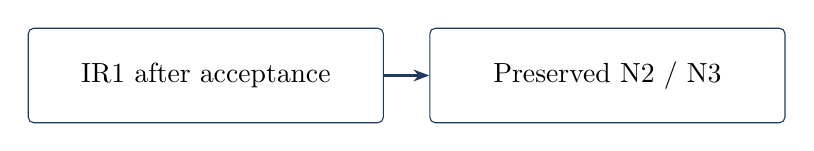
\begin{tikzpicture}[y=.70cm]
\node[box,font=\normalsize,text width=43mm,minimum height=12mm] (a0) at (0.0,0) {IR1 after acceptance};
\node[box,font=\normalsize,text width=43mm,minimum height=12mm] (a1) at (5.1,0) {Preserved N2 / N3};
\draw[flow] (a0.east) -- (a1.west);\end{tikzpicture}\par\medskip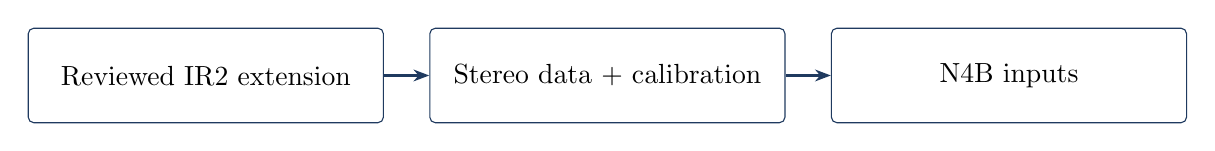
\begin{tikzpicture}[y=.70cm]
\node[box,font=\normalsize,text width=43mm,minimum height=12mm] (a0) at (0.0,0) {Reviewed IR2 extension};
\node[box,font=\normalsize,text width=43mm,minimum height=12mm] (a1) at (5.1,0) {Stereo data + calibration};
\draw[flow] (a0.east) -- (a1.west);
\node[box,font=\normalsize,text width=43mm,minimum height=12mm] (a2) at (10.2,0) {N4B inputs};
\draw[flow] (a1.east) -- (a2.west);\end{tikzpicture}}{Stereo extension; schematic.}
\vfill\takeaway{The stereo goal does not authorize quietly changing N2.}
\note{An IR1-only dataset cannot feed stereo-inertial estimation. Prepare a separately reviewed extension with both camera projections, stereo extrinsics/rectification, all required motion/time coverage, explicit topics and lossless data. Existing mono-inertial candidate artifacts are not stereo qualification. Source register: B,G,O. PLANNED separately reviewed IR2 profile/topic/storage/calibration extension precedes N4B; accepted IR1-only N2/N3 stay intact.}\end{frame}
\begin{frame}{4.9 N4A: camera-independent EuRoC baseline}\evidence{MEASURED trials / gate OPEN}
Entry: N0 only in the camera gate graph; separately authorized ORB run, pinned isolated build, dataset/settings hashes. No N1--N3 dependency.\begin{block}{Future commands / tools}{\ttfamily\normalsize cmake --build "\$WBR\_ORB\_WORK/build" \textbackslash{}\par \quad --target stereo\_inertial\_euroc --parallel 2\par ./Examples/Stereo-Inertial/stereo\_inertial\_euroc \textbackslash{}\par \quad Vocabulary/ORBvoc.txt SETTINGS.yaml SEQUENCE TIMES.txt RUN\_ID}\end{block}\medskip Build dependencies in the documented stages first. Freeze stereo settings and dataset reference coverage. Retain compile/run logs, initialization events, f\_RUN\_ID.txt and kf\_RUN\_ID.txt.\par\medskip\textbf{Measured baseline}: Three MH01 runs: one map, no resets, IMU initialized. Accuracy is measured; power, local-error checks and budgets leave N4A OPEN.\par\vfill\takeaway{Known-data accuracy supports this build; acceptance remains OPEN.}\note{Source: docs/ORB\_SLAM3\_OFFLINE\_PREPARATION.md; upstream pinned stereo\_inertial\_euroc.cc. Commands are teaching examples only; none executed. UNKNOWN budgets require approval.}\note{Merged original page 15: 
\deckitems{\item EuRoC micro aerial vehicle data contain stereo images and IMU. \hyperlink{referencepage}{[2]} \item Published reference trajectories support algorithm evaluation.\item Freeze sequence, calibration and reference association policy.\item A dataset baseline does not qualify Pi camera transport.}
\vfill
\begin{block}{Engineering decision}Compare build/configuration and estimator behavior before involving live capture.\end{block}
\vfill\takeaway{Use known inputs to isolate build and estimator problems.}
Burri et al., 2016. EuRoC references have sequence-dependent motion-capture/laser-tracker limitations. Read known issues and use compatible reference coverage. No dataset download, build or ORB execution is authorized by this deck task. Source register: EU,P. EuRoC micro aerial vehicle data provide stereo, IMU and reference trajectories; these are published dataset properties, not Pi results.}\end{frame}
\begin{frame}{4.9 N4A: estimator acceptance contract}\evidence{PLANNED / no gate PASS}
Absolute Trajectory Error (ATE) scores aligned paths; Relative Pose Error (RPE) scores motion increments.\par\medskip\begin{tabular}{@{}L{65mm}L{77mm}L{38mm}@{}}\toprule
\textbf{Required / open threshold} & \textbf{Measurement / clock} & \textbf{Proposed evidence}\\\midrule
Finite ordered trajectories; coverage & Export epochs in dataset time; coordinate/format audit & Trajectory files + audit\\[6pt]
Repeat initialization / tracking & All attempts incl. failure; first eligible dataset epoch + host events & Run/state timelines\\[6pt]
Accuracy / continuity budgets UNKNOWN & Reference association, rigid alignment, ATE/RPE; dataset epochs & evo outputs + budget review\\[6pt]
\bottomrule\end{tabular}\par\medskip FAIL: load/link error $\to$ build; empty images $\to$ reader paths; no inertial initialization $\to$ settings/time/motion. No accepted numeric budget means no performance PASS. N4A also lacks stable-power reruns and RPE.\vfill\takeaway{MH01 accuracy is measured; N0 power health and this contract remain incomplete.}\note{Source: docs/ORB\_SLAM3\_OFFLINE\_PREPARATION.md; upstream pinned stereo\_inertial\_euroc.cc. Commands are teaching examples only; none executed. UNKNOWN budgets require approval.}\end{frame}
\begin{frame}{4.10 N4B: offline D435i stereo}\evidence{MEASURED build / camera run OPEN}
\begin{block}{Entry remains conditional}N3 plus reviewed IR2 stereo extension, accepted calibration and qualified data storage. The direct SDK candidate does not bypass these gates.\end{block}\begin{block}{Prepared candidate}\texttt{d435i\_record} writes stereo/motion to \texttt{stereo\_imu.db3} and \texttt{timestamps.csv}. The patched D435i example reads it with \texttt{--bag FILE --no-viewer}.\end{block}\medskip Both binaries are built; neither has run on this camera. Native SDK replay is the present candidate; a separate ROS stereo conversion path remains PLANNED.\vfill\takeaway{Build and linkage establish executable readiness, not N4B input or estimator acceptance.}\note{Evidence: experiments/2026-10-13-SESSION\_FACTS\_FOR\_SLIDES.md; experiments/2026-10-13-n4b-d435i-prep/n4b\_plan.md. Deck authoring only; no camera, Pi or ORB program was executed in Phase 6.}\end{frame}
\begin{frame}{4.10 N4B: input and run criteria}\evidence{PLANNED / no gate PASS}
\par\begin{tabular}{@{}L{63mm}L{79mm}L{38mm}@{}}\toprule
\textbf{Required / open threshold} & \textbf{Measurement / clock} & \textbf{Proposed evidence}\\\midrule
Lossless stereo + valid pairing & Counts/pixels, epipolar residuals, left/right stamp difference; source domain & Association / image audit\\[6pt]
Calibrated geometry, noise and offset & Holdout residuals; camera/IMU units and common time relation & Calibration report + hashes\\[6pt]
Repeatable finite tracking; budgets UNKNOWN & All trials, epochs, initialization/loss; no GT means accuracy UNKNOWN & Run logs + trajectories\\[6pt]
\bottomrule\end{tabular}\par\medskip FAIL: vertical mismatch $\to$ rectification; missing brackets $\to$ motion coverage; bias instability $\to$ clocks/calibration before feature tuning. Residual limits are not yet approved.\vfill\takeaway{Default/CAD values and zero placeholder noise do not qualify final VIO.}\note{Source: docs/ORB\_SLAM3\_OFFLINE\_PREPARATION.md; upstream pinned stereo\_inertial\_euroc.cc. Commands are teaching examples only; none executed. UNKNOWN budgets require approval.}\end{frame}
\begin{frame}{4.10 N4B: immutable adapter provenance}\evidence{MEASURED binary build / replay OPEN}
\begin{columns}[T,onlytextwidth]\begin{column}{.48\textwidth}\begin{block}{Derived input contract}Preserve raw bags. Manifest links input, converter, settings and calibration hashes; record domains, offset sign, interpolation brackets and every rejected sample.\end{block}\end{column}\begin{column}{.48\textwidth}\coursefigure{P10}{\slideimg[.46\textheight]{\linewidth}{P10}{Offline frozen-input analysis}}{Frozen inputs make estimator comparisons attributable.}\end{column}\end{columns}\vfill\takeaway{In Figure~\ref{fig:P10}, test lossless pixels, exact nanoseconds, no extrapolation and count reconciliation.}\note{Source: docs/ORB\_SLAM3\_OFFLINE\_PREPARATION.md; upstream pinned stereo\_inertial\_euroc.cc. Commands are teaching examples only; none executed. UNKNOWN budgets require approval.}\end{frame}
\begin{frame}{4.11 N4C: live stereo scheduling}\evidence{MEASURED build / live run OPEN}
\begin{columns}[T,onlytextwidth]\begin{column}{.48\textwidth}\begin{block}{Entry / purpose}Accepted N4B evidence, renewed N1--N3 under stereo load, unchanged settings/calibration. Isolate live scheduling from input defects.\end{block}\end{column}\begin{column}{.48\textwidth}\begin{block}{Prepared candidate}The same patched \texttt{stereo\_inertial\_realsense\_D435i} binary reads the camera when \texttt{--bag} is omitted. \texttt{--no-viewer} disables the display.\end{block}\end{column}\end{columns}\medskip Built, never run on this camera. Queue bounds, initialization/loss traces, valid time domains and source age remain unmeasured. A ROS live bridge is still PLANNED.\vfill\takeaway{A working executable cannot establish live freshness or sustained throughput.}\note{Evidence: experiments/2026-10-13-SESSION\_FACTS\_FOR\_SLIDES.md; experiments/2026-10-13-n4b-d435i-prep/n4b\_plan.md. Deck authoring only; no camera, Pi or ORB program was executed in Phase 6.}\end{frame}
\begin{frame}{4.11 N4C: live PASS/FAIL criteria}\evidence{PLANNED / no gate PASS}
\par\begin{tabular}{@{}L{65mm}L{77mm}L{38mm}@{}}\toprule
\textbf{Required / open threshold} & \textbf{Measurement / clock} & \textbf{Proposed evidence}\\\midrule
Valid paired input + IMU coverage & Source epochs; renewed stereo transport metrics & Input / pairing timeline\\[6pt]
Initialization / continuity budgets UNKNOWN & Attempt count; loss/reset state; source epochs + host event times & State timeline / trajectories\\[6pt]
Latency / queue bounds UNKNOWN & Queue, compute, receipt/output on host steady; mapped capture with uncertainty & Latency / queue / health log\\[6pt]
\bottomrule\end{tabular}\par\medskip FAIL: offline works, live lags $\to$ wrapper/DDS/executor/queue; thermal stalls $\to$ N0 under load; loss in both $\to$ input/calibration first. Missing counters stay UNKNOWN.\vfill\takeaway{Approve bounds before a live performance verdict; do not tune around unmeasured age.}\note{Source: docs/ORB\_SLAM3\_OFFLINE\_PREPARATION.md; upstream pinned stereo\_inertial\_euroc.cc. Commands are teaching examples only; none executed. UNKNOWN budgets require approval.}\end{frame}
\begin{frame}{4.12 N5: reproducible measurement}\evidence{PLANNED / no gate PASS}
Entry: qualified N4 trials, frozen hypotheses, trial count, reference and clock relations. Retain failures; at least three offline repeats is a PLANNED minimum.\begin{block}{Future commands / tools}{\ttfamily\normalsize evo\_ape tum REFERENCE.tum ESTIMATE.tum --align\par evo\_rpe tum REFERENCE.tum ESTIMATE.tum --help}\end{block}\begin{columns}[T,onlytextwidth]\begin{column}{.48\textwidth}\begin{block}{Outputs}Original exports, conversion audit, evo version/argv/results, latency samples with eligibility, initialization/loss events and resource time series.\end{block}\end{column}\begin{column}{.48\textwidth}\begin{block}{Tools still planned}Event instrumentation and queue counters need reviewed implementation. No first-party N5 acceptance validator exists. Approve metric bounds before the campaign.\end{block}\end{column}\end{columns}\vfill\takeaway{A metric file is a measurement artifact, not automatic performance acceptance.}\note{Source: docs/ORB\_SLAM3\_OFFLINE\_PREPARATION.md; upstream pinned stereo\_inertial\_euroc.cc; evo maintainer Metrics [8]. Commands are teaching examples only; none executed. UNKNOWN budgets require approval.}\end{frame}
\begin{frame}{4.12 N5: measurement criteria}\evidence{PLANNED / no gate PASS}
\par\begin{tabular}{@{}L{61mm}L{79mm}L{40mm}@{}}\toprule
\textbf{Required / open threshold} & \textbf{Measurement / clock} & \textbf{Proposed evidence}\\\midrule
ATE/RPE only with valid reference & Associated source epochs; rigid alignment; overlap and exclusions & evo raw output / audit\\[6pt]
P50/P95/P99 + initialization/loss & Named interval, estimator and sample count; host steady / source epochs & Raw events + trial summary\\[6pt]
Resources, losses, queue depth & One-Hz health + event join; sequence/count reconciliation; unknown counters marked & Health / counter time series\\[6pt]
\bottomrule\end{tabular}\par\medskip All numeric performance budgets are UNKNOWN. FAIL: cross-domain subtraction $\to$ clocks; suspicious low ATE $\to$ alignment/association; averages hide stalls $\to$ raw timeline.\par\medskip\textbf{Continuity denominator}: Count all initialization attempts; define first eligible input. Record state, reset/session ID, loss intervals and trajectory coverage.\par\vfill\takeaway{Missing ground truth blocks accuracy claims; it does not force synthetic zero errors.}\note{Source: docs/ORB\_SLAM3\_OFFLINE\_PREPARATION.md; upstream pinned stereo\_inertial\_euroc.cc. Commands are teaching examples only; none executed. UNKNOWN budgets require approval.}\note{Merged original page 93: 
\deckitems{\item Success rate uses all declared initialization attempts as denominator.\item Measure initialization time from a defined first eligible input.\item Track loss duration, resets and relocalization events.\item Check trajectory coverage, not only exported sample count.}
\vfill
\begin{tabular}{L{87.0mm}L{87.0mm}}\toprule
\textbf{Event record} & \textbf{Required interpretation}\\\midrule
First eligible input & Initialization-time origin\\[5pt]
Tracking state / reset & Continuity and loss intervals\\[5pt]
Pose epoch / output time & Coverage versus freshness\\[5pt]
\bottomrule\end{tabular}
\vfill\takeaway{Report failed attempts alongside successful trajectories.}
Retain sensor epoch, local event time, state, reset/session/map identifier and exclusion reason. Pose export presence alone cannot recover all state events. Numerical state-event instrumentation and interface changes require review before implementation. Source register: O,U. Success denominator, initialization time, tracking loss duration, resets and relocalization need preserved state events and failed trials.}\end{frame}
\begin{frame}{4.13 N6: health semantics with fixtures}\evidence{PLANNED / no gate PASS}
\begin{columns}[T,onlytextwidth]\begin{column}{.48\textwidth}\begin{block}{Entry / purpose}Reviewed message semantics after N5; rate, transport, age rule and clock relation approved. Use synthetic fixtures before hardware integration.\end{block}\end{column}\begin{column}{.48\textwidth}\begin{block}{Tools / evidence}PLANNED receiver harness; no runnable project validator exists. Deliver event fixtures, expected/actual transitions, rejection reasons and revision hashes.\end{block}\end{column}\end{columns}\par\begin{tabular}{@{}L{85mm}L{99mm}@{}}\toprule
\textbf{Fixture} & \textbf{Expected planned response}\\\midrule
Old epoch + fresh heartbeat & STALE; heartbeat does not refresh pose\\[6pt]
New boot / reset / map ID & Re-establish session and frame\\[6pt]
NaN, wrong frame, duplicate sequence & INVALID / reject; optional input withdrawn\\[6pt]
\bottomrule\end{tabular}\par\vfill\takeaway{Synthetic health tests qualify semantics only; they do not prove robot fallback.}\note{Source: docs/ARCHITECTURE.md; docs/DECISIONS.md. Commands are teaching examples only; none executed. UNKNOWN budgets require approval.}\end{frame}
\begin{frame}{4.13 N6: planned acceptance table}\evidence{PLANNED / no gate PASS}
\par\begin{tabular}{@{}L{64mm}L{77mm}L{39mm}@{}}\toprule
\textbf{PASS contract / open threshold} & \textbf{Measurement / clock} & \textbf{Proposed evidence}\\\midrule
Reject every declared invalid fixture & Compare expected/actual state + reason; synthetic event time & Fixture verdicts\\[6pt]
Age bound $\leq A_{max}$; value UNKNOWN & Source-age bound + receiver elapsed time; defined Pi/STM32 relation & Clock / wrap / delay fixtures\\[6pt]
Reset re-establishment explicit & Session/frame sequence; no silent recovery & Transition trace + review\\[6pt]
\bottomrule\end{tabular}\par\medskip FAIL: old pose accepted $\to$ source-age semantics; wrap breaks timeout $\to$ receiver clock; old session accepted $\to$ reset protocol. Rate and timeout remain unselected.\vfill\takeaway{Implement only after API/message review; do not infer acceptance from a heartbeat.}\note{Source: docs/ARCHITECTURE.md. Commands are teaching examples only; none executed. UNKNOWN budgets require approval.}\end{frame}
\begin{frame}{4.14 N7: staged controller boundary}\evidence{PLANNED / no gate PASS}
\begin{columns}[T,onlytextwidth]\begin{column}{.48\textwidth}\begin{block}{Entry / purpose}N6 semantics accepted plus separate safety authorization. STM32 body IMU, control loops, watchdog and motor limits remain local.\end{block}\end{column}\begin{column}{.48\textwidth}\begin{block}{Tools / artifacts}PLANNED bench receiver / controlled fault injection; no approved motor-test command exists. Preserve STM32 and Pi traces, test setup, fallback policy and safety review.\end{block}\end{column}\end{columns}\par\begin{tabular}{@{}L{67mm}L{117mm}@{}}\toprule
\textbf{Stage} & \textbf{Evidence needed before progression}\\\midrule
Receiver bench, no actuation & Link loss, stale/reset/invalid rejection\\[6pt]
Approved controlled integration & Local balance timing and watchdog independence\\[6pt]
Separately approved physical test & Safe setup; controller-owned fallback observations\\[6pt]
\bottomrule\end{tabular}\par\vfill\takeaway{Pi loss must not remove local balance authority; actual stability is unmeasured.}\note{Source: AGENTS.md; docs/ARCHITECTURE.md. Commands are teaching examples only; none executed. UNKNOWN budgets require approval.}\end{frame}
\begin{frame}{4.14 N7: planned acceptance table}\evidence{PLANNED / no gate PASS}
\par\begin{tabular}{@{}L{62mm}L{77mm}L{41mm}@{}}\toprule
\textbf{Required / open threshold} & \textbf{Measurement / clock} & \textbf{Proposed evidence}\\\midrule
No perception authority over safety & Ownership / code review + controlled fault trace & Boundary review\\[6pt]
Local control retained on Pi loss & STM32 loop/watchdog/motor state; MCU clock & Controller trace + setup\\[6pt]
Fallback inside approved safety budget & Fault onset to local action; MCU domain; numeric bound UNKNOWN & Fault timeline + sign-off\\[6pt]
\bottomrule\end{tabular}\par\medskip FAIL: balance depends on ROS heartbeat $\to$ ownership; stale reference retained $\to$ fallback semantics; link reset bypasses validation $\to$ session handling.\vfill\takeaway{No approved setup and bound means no physical integration PASS.}\note{Source: AGENTS.md; docs/ARCHITECTURE.md. Commands are teaching examples only; none executed. UNKNOWN budgets require approval.}\end{frame}
\begin{frame}{4.15 Reproduction and evidence}\evidence{PLANNED}
\deckitems{\item Build a new checksummed bundle from canonical Mac utilities. (Figure~\ref{fig:D64})\item Deploy into a new Pi runtime directory; verify hashes there.\item Store exact commands, settings, logs and real review receipts.\item Retain historical evidence and every failed run unchanged.}
\vfill
\coursefigure{D64}{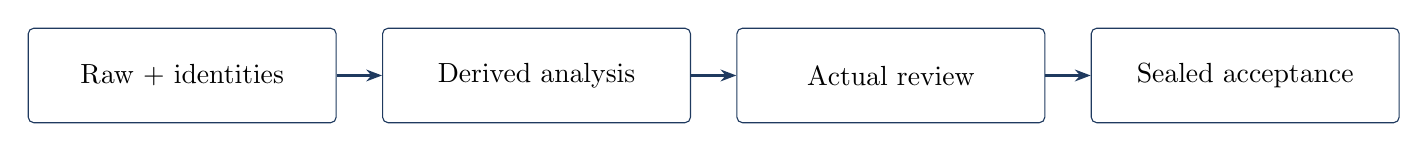
\begin{tikzpicture}[y=.70cm]
\node[box,font=\normalsize,text width=37.0mm,minimum height=12mm] (a0) at (0.0,0) {Raw + identities};
\node[box,font=\normalsize,text width=37.0mm,minimum height=12mm] (a1) at (4.5,0) {Derived analysis};
\draw[flow] (a0.east) -- (a1.west);
\node[box,font=\normalsize,text width=37.0mm,minimum height=12mm] (a2) at (9.0,0) {Actual review};
\draw[flow] (a1.east) -- (a2.west);
\node[box,font=\normalsize,text width=37.0mm,minimum height=12mm] (a3) at (13.5,0) {Sealed acceptance};
\draw[flow] (a2.east) -- (a3.west);\end{tikzpicture}}{Reproduction and evidence; schematic.}
\par\medskip\textbf{Acceptance receipt}: Require actual log/image review and recomputed sealed evidence; retain calibration warnings.\par\vfill\takeaway{A reviewable evidence packet is the deliverable of each gate.}
\note{Raw records precede derived analysis and explicit human acceptance. Do not fabricate review.json booleans or modify deployed sources in place. Bundle manifests include dirty-source hashes; successful software tests are labeled offline/synthetic tooling only. Source register: G,T. Deploy new checksummed Mac bundles; retain full commands/config/raw logs/review receipts; never reset checkouts.}\note{Merged original page 62: 
\begin{block}{Future commands / tools}{\ttfamily\normalsize python3 phase\_gate.py accept-n2 --camera-available \textbackslash{}\par \quad --n1-result "\$WBR\_RUN/n1/result.json" \textbackslash{}\par \quad --smoke "\$WBR\_RUN/smoke/capture-result.json" \textbackslash{}\par \quad --reproduction "\$WBR\_RUN/reproduction/capture-result.json" \textbackslash{}\par \quad --soak "\$WBR\_RUN/soak/capture-result.json" \textbackslash{}\par \quad --review "\$WBR\_RUN/review.json" --output "\$WBR\_RUN/n2-accepted"}\end{block}\medskip Review.json must reflect actual log/image inspection and calibration provenance. Never prefill acceptance booleans. Sealed evidence is recomputed, not merely trusted.\vfill\takeaway{N2 transport acceptance still leaves final VIO calibration blocked.}Source: experiments/2026-09-12-pi5-native-sensor-validation/PHASE\_A\_RUNBOOK.md. Commands are teaching examples only; none executed. UNKNOWN budgets require approval.}\end{frame}
\begin{frame}{4.16 Bottom-up diagnosis}\evidence{KNOWN debugging order / PLANNED runs}
\deckitems{\item Inspect hardware, power and the camera’s own USB branch first. (Figure~\ref{fig:D65})\item Then raw streams, clocks, driver, ROS graph and QoS.\item Then calibration, ORB input/state, trajectory and evaluation.\item Fix the earliest failed layer; preserve downstream symptoms.}
\vfill
\coursefigure{D65}{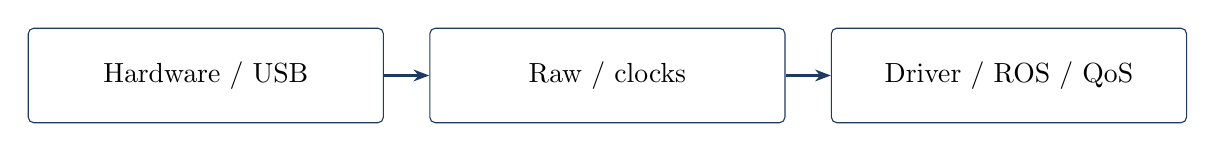
\begin{tikzpicture}[y=.70cm]
\node[box,font=\normalsize,text width=43mm,minimum height=12mm] (a0) at (0.0,0) {Hardware / USB};
\node[box,font=\normalsize,text width=43mm,minimum height=12mm] (a1) at (5.1,0) {Raw / clocks};
\draw[flow] (a0.east) -- (a1.west);
\node[box,font=\normalsize,text width=43mm,minimum height=12mm] (a2) at (10.2,0) {Driver / ROS / QoS};
\draw[flow] (a1.east) -- (a2.west);\end{tikzpicture}\par\medskip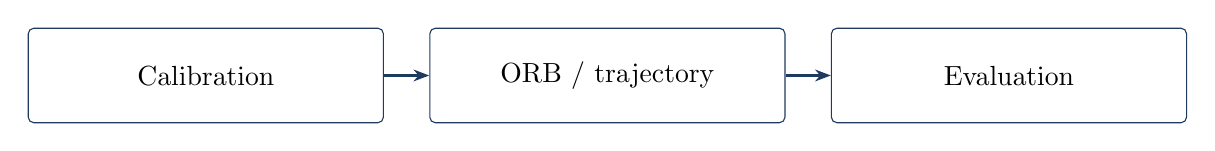
\begin{tikzpicture}[y=.70cm]
\node[box,font=\normalsize,text width=43mm,minimum height=12mm] (a0) at (0.0,0) {Calibration};
\node[box,font=\normalsize,text width=43mm,minimum height=12mm] (a1) at (5.1,0) {ORB / trajectory};
\draw[flow] (a0.east) -- (a1.west);
\node[box,font=\normalsize,text width=43mm,minimum height=12mm] (a2) at (10.2,0) {Evaluation};
\draw[flow] (a1.east) -- (a2.west);\end{tikzpicture}}{Bottom-up diagnosis; schematic.}
\par\medskip\textbf{Symptoms}: 480M: cable/branch/power. Topic silence: graph/readback/QoS. Initialization failure: pairing, motion, frames, offset/noise.\par\vfill\takeaway{Do not tune SLAM to hide a transport failure.}
\note{Bottom-up order reduces ambiguity. Save complete logs before changing one variable. Use recorded inputs to separate acquisition from estimator behavior; add only instrumentation needed to answer the bounded question. Source register: A,H,G. Hardware$\rightarrow$USB$\rightarrow$raw$\rightarrow$clocks$\rightarrow$driver$\rightarrow$ROS$\rightarrow$QoS$\rightarrow$calibration$\rightarrow$ORB-SLAM3$\rightarrow$trajectory$\rightarrow$evaluation; fix first failed layer.}\note{Merged original page 85: 
\deckitems{\item 480M: inspect cable, direct branch and power before software.\item Silent topic: inspect publisher, parameter readback and QoS.\item Initialization failure: inspect coverage, frames, offset and noise.\item Calibration fallback: preserve warning; do not copy constants.}
\vfill
\begin{tabular}{L{87.0mm}L{87.0mm}}\toprule
\textbf{Symptom} & \textbf{First discriminating evidence}\\\midrule
480M / disconnect & Own branch + power/kernel logs\\[5pt]
Topic silence & Graph + readback + QoS\\[5pt]
Loss / failed initialization & Pairing + motion coverage + calibration\\[5pt]
\bottomrule\end{tabular}
\vfill\takeaway{Similar symptoms can require different evidence.}
Permissions need exact device-ancestor inspection, not broad access. If trajectory looks smooth, still inspect stale epochs, reset state and reference coverage. A storage bottleneck can manifest as delayed recording without raw sensor failure. Diagnose one layer at a time. Source register: H,E,C. USB2/power/permissions/topic silence/bad association/calibration fallback need different evidence and remedies.}\end{frame}
\begin{frame}{4.18 Bounded AI tickets}\evidence{PLANNED}
\begin{columns}[T,onlytextwidth]\begin{column}{.48\textwidth}\deckitems{\item Artificial intelligence (AI): one bounded question. (Figure~\ref{fig:P11})\item Limit files, hosts, actions and fixtures.\item Require commands, evidence and STOP conditions.\item Owner accepts gates and safety decisions.}\end{column}\begin{column}{.48\textwidth}
\coursefigure{P11}{\slideimg[.49\textheight]{\linewidth}{P11}{Bounded engineering task packet}}{Bounded engineering task packet; conceptual.}\end{column}\end{columns}
\vfill\takeaway{Delegate analysis, not unbounded authority.}
\note{Gate tickets: N0 inventory; N1 own-branch/access diagnosis; N2 sealed timing/content recomputation; N3 context/replay checks; N4 settings/association/fixed-data run; N5 metrics; N6 reviewed semantic fixtures; N7 approved boundary documentation. Do not delegate guessed calibration, blanket reinstall, fabricated review or autonomous motor tests. Source register: R,T,O. Artificial intelligence (AI) agents get one uncertainty, allowed files/actions, fixtures, evidence and stop conditions; owner accepts gates.}\end{frame}
\begin{frame}{5.2 ATE computation outline}\evidence{PLANNED / no gate PASS}
Absolute Trajectory Error (ATE) compares associated poses after a declared alignment. $P_i$ is the estimate and $Q_i$ the reference; root mean square error (RMSE) summarizes translation [8].\par\medskip\coursefigure{D70}{
\begin{tikzpicture}[y=.8cm,font=\normalsize,box/.append style={font=\normalsize}]\node[box,text width=165mm] {$E_i=Q_i^{-1}SP_i,\qquad e_i=\|\operatorname{trans}(E_i)\|,\qquad \mathrm{RMSE}=\sqrt{\frac{1}{N}\sum_i e_i^2}$};\end{tikzpicture}}{Rigid alignment S removes reference-origin choice, not a stereo scale error.}\par\medskip Associate epochs within a predeclared tolerance; retain unmatched samples. Convert both trajectories to the same pose direction and units before fitting $S$. Report valid overlap and failure trials.\vfill\takeaway{In Figure~\ref{fig:D70}, without independent reference data, D435i absolute accuracy stays UNKNOWN.}\note{Source: docs/ORB\_SLAM3\_OFFLINE\_PREPARATION.md; upstream pinned stereo\_inertial\_euroc.cc; evo Metrics. Commands are teaching examples only; none executed. UNKNOWN budgets require approval.}\end{frame}
\begin{frame}{5.3 RPE and pair policy}\evidence{PLANNED / no gate PASS}
Relative Pose Error (RPE) compares estimated motion with reference motion over a declared interval [8].\par\medskip\coursefigure{D71}{
\begin{tikzpicture}[y=.8cm,font=\normalsize,box/.append style={font=\normalsize}]\node[box,text width=165mm] {$E_{ij}=(Q_i^{-1}Q_j)^{-1}(P_i^{-1}P_j)$\\Translation and rotation are separate metrics.};\end{tikzpicture}}{Relative deltas expose local drift rather than global alignment choice.}\par\par\begin{tabular}{@{}L{83mm}L{101mm}@{}}\toprule
\textbf{Pair policy} & \textbf{Question answered}\\\midrule
Fixed time separation & How wrong is motion over that duration?\\[6pt]
Fixed distance separation & How does error grow per traveled distance?\\[6pt]
Consecutive vs all eligible pairs & Different weighting; report choice and pair count\\[6pt]
\bottomrule\end{tabular}\par\vfill\takeaway{In Figure~\ref{fig:D71}, never compare RPE numbers with different delta units or pairing policies.}\note{Source: evo Metrics [8]. Commands are teaching examples only; none executed. UNKNOWN budgets require approval.}\end{frame}
\begin{frame}{5.4 Trajectory conversion and evo}\evidence{PLANNED / no gate PASS}
\begin{block}{Future commands / tools}{\ttfamily\normalsize evo\_ape tum REFERENCE.tum ESTIMATE.tum --align\par evo\_rpe tum REFERENCE.tum ESTIMATE.tum \textbackslash{}\par \quad --pose\_relation angle\_deg --delta 1 --delta\_unit m}\end{block}\medskip The 1 m delta is a command example, not a project acceptance threshold [8]. Check installed --help, version, association tolerance, valid coverage and reference quality.\begin{block}{Conversion before comparison}Technical University of Munich (TUM) format uses seconds, xyz and quaternion qx qy qz qw. Preserve EuRoC originals; audit quaternion order, units, pose direction and frame. Metric stereo defaults to rigid alignment; scale fitting is a separate diagnostic.\end{block}\vfill\takeaway{Store exact argv and raw output; conversion errors can dominate the metric.}\note{Source: docs/ORB\_SLAM3\_OFFLINE\_PREPARATION.md; upstream pinned stereo\_inertial\_euroc.cc; evo Metrics/Formats. Commands are teaching examples only; none executed. UNKNOWN budgets require approval.}\end{frame}
\begin{frame}{5.6 Latency and loss}\evidence{PLANNED}
\deckitems{\item P50/P95/P99 are the 50th/95th/99th latency percentiles.\item Name receipt-to-start, processing and receipt-to-output separately.\item Reconcile sequence gaps, received counts and recorded counts.\item Unavailable queue/drop counters remain UNKNOWN.}
\vfill
\begin{tabular}{L{87.0mm}L{87.0mm}}\toprule
\textbf{Metric} & \textbf{Required evidence}\\\midrule
Latency percentiles & Named interval / clock / count\\[5pt]
Loss & Sequence and count reconciliation\\[5pt]
Queue depth / drops & Measured counter or UNKNOWN\\[5pt]
\bottomrule\end{tabular}
\vfill\takeaway{Percentiles need event definitions and eligible sample counts.}
\note{Use one monotonic clock for host intervals. Capture-to-output requires mapping uncertainty. Define percentile estimator, warmup policy and number of samples. Frame loss, delayed arrival and intentional input rejection are different events; do not call all count mismatches dropped frames. Source register: B,G,C. P50/P95/P99 percentiles use named same-clock intervals; sequence/count gaps and unavailable queue/drop counters stay distinct.}\end{frame}
\begin{frame}{5.7 Resource measurements}\evidence{PLANNED}
\deckitems{\item Log Central Processing Unit (CPU) load and clock frequency. (Figure~\ref{fig:D75})\item Track temperature, memory and Resident Set Size (RSS).\item Record throttling, queue depth and free data space.\item Align samples with initialization, loss and optimization events.}
\vfill
\coursefigure{D75}{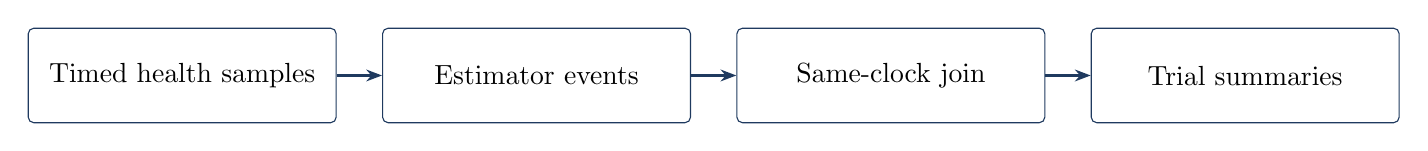
\begin{tikzpicture}[y=.70cm]
\node[box,font=\normalsize,text width=37.0mm,minimum height=12mm] (a0) at (0.0,0) {Timed health samples};
\node[box,font=\normalsize,text width=37.0mm,minimum height=12mm] (a1) at (4.5,0) {Estimator events};
\draw[flow] (a0.east) -- (a1.west);
\node[box,font=\normalsize,text width=37.0mm,minimum height=12mm] (a2) at (9.0,0) {Same-clock join};
\draw[flow] (a1.east) -- (a2.west);
\node[box,font=\normalsize,text width=37.0mm,minimum height=12mm] (a3) at (13.5,0) {Trial summaries};
\draw[flow] (a2.east) -- (a3.west);\end{tikzpicture}}{Resource measurements; schematic.}
\vfill\takeaway{Resource averages cannot explain tail stalls alone.}
\note{Use system and process CPU separately, sample cadence, host-steady timestamps and complete hardware health logs. Frequencies/temperature are observations, not electrical power measurements. Unsupported queue instrumentation stays unknown. Capture tools themselves contribute overhead. Source register: T,O. Log Central Processing Unit (CPU) load/frequency, temperature, memory, Resident Set Size (RSS), throttling and queue depth against events.}\end{frame}
\begin{frame}{5.8 Accuracy results}\evidence{MEASURED N4A / SOURCE-SUPPORTED paper}
N4A: MH01, rigid alignment, body poses; 0.02 s association tolerance. [1,8]\par\medskip\par\medskip\coursefigure{D76}{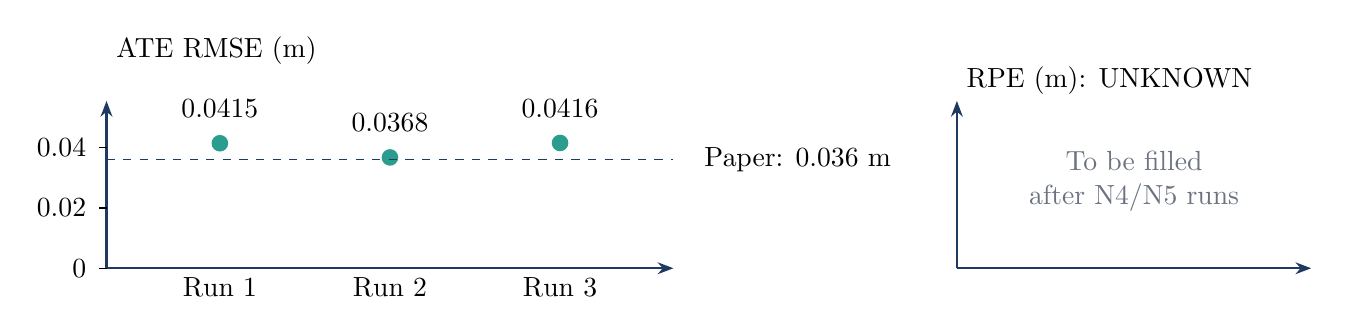
\begin{tikzpicture}[x=.90cm,y=.85cm,font=\normalsize,box/.append style={font=\normalsize}]
\draw[flow] (0,0)--(8,0);\draw[flow] (0,0)--(0,2.5);
\foreach \y/\lab in {0/0,.9/0.02,1.8/0.04}{\draw (0,\y)--(-.1,\y);\node[anchor=east] at (-.15,\y){\lab};}
\node[anchor=west] at (0,3.25){ATE RMSE (m)};
\foreach \x/\y/\val/\run in {1.6/1.8675/0.0415/1,4/1.656/0.0368/2,6.4/1.872/0.0416/3}{\fill[teal] (\x,\y) circle (3pt);\node[above=2mm] at (\x,\y){\val};\node[below] at (\x,0){Run \run};}
\draw[dashed,navy] (0,1.62)--(8,1.62);\node[anchor=west] at (8.3,1.62){Paper: 0.036 m};
\draw[flow] (12,0)--(17,0);\draw[flow] (12,0)--(12,2.5);\node[anchor=west] at (12,2.8){RPE (m): UNKNOWN};
\node[text width=49mm,align=center,text=muted] at (14.5,1.3){To be filled\\after N4/N5 runs};
\end{tikzpicture}}{N4A measured ATE; the dashed line is published, not our measurement.}\par\medskip Mean: 0.040 m (4.0 cm). Paper Table II: 0.036 m, median of ten trials. D435i accuracy and N4A RPE remain UNKNOWN.\vfill\takeaway{Similar magnitude on MH01 supports the build; it does not qualify the robot. (Figure~\ref{fig:D76})}\note{Evidence: experiments/2026-10-13-n4a-euroc-mh01/REPORT.md; Campos et al., arXiv:2007.11898v2 Table II (verified 2026-10-13). Deck authoring only; no camera, Pi or ORB program was executed in Phase 6.}\end{frame}
\begin{frame}{5.9 Timing results}\evidence{MEASURED wall durations / timing qualification OPEN}
N4A wall durations: 301 / 282 / 284 s for 184 s of dataset time. These include vocabulary load; live under-voltage invalidates a speed verdict.\par\medskip\par\medskip\coursefigure{D77}{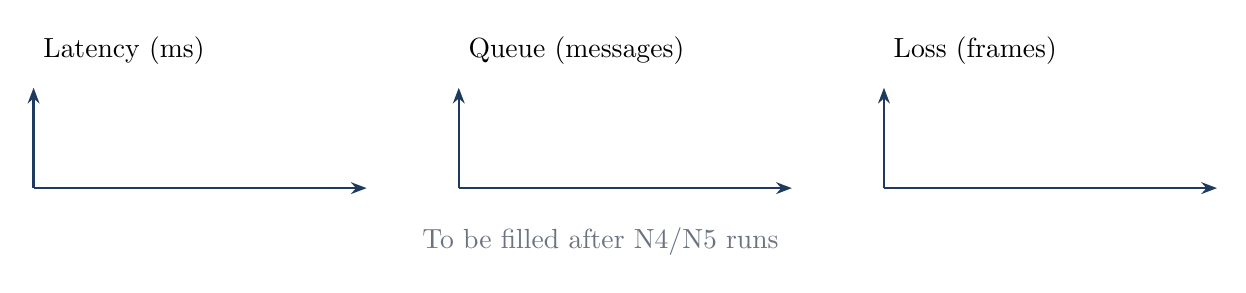
\begin{tikzpicture}[x=.90cm,y=.85cm,font=\normalsize,box/.append style={font=\normalsize}]
\foreach \x/\lab in {0/Latency (ms),6/Queue (messages),12/Loss (frames)}{\draw[flow] (\x,0)--(\x+4.7,0);\draw[flow] (\x,0)--(\x,1.5);\node[anchor=south west] at (\x,1.7){\lab};}
\node[text=muted] at (8,-.8){To be filled after N4/N5 runs};
\end{tikzpicture}}{Wall duration is observed; per-frame latency, queues and loss remain unmeasured.}\par\medskip Do not convert wall duration into P50/P95/P99 processing latency. Separate startup, steady tracking and shutdown on a stable-power rerun.\vfill\takeaway{Offline completion and real-time processing answer different questions. (Figure~\ref{fig:D77})}\note{Evidence: experiments/2026-10-13-n4a-euroc-mh01/REPORT.md. Deck authoring only; no camera, Pi or ORB program was executed in Phase 6.}\end{frame}
\begin{frame}{5.10 Resource results}\evidence{MEASURED N4A summaries / missing series UNKNOWN}
\par\begin{tabular}{@{}L{83mm}L{101mm}@{}}\toprule\textbf{N4A observed summary} & \textbf{Value / interpretation}\\\midrule
Peak process RSS, runs 1 / 2 / 3 & 823 / 828 / 828 MiB\\[6pt]Live under-voltage / throttling & 87 / 178 five-second samples = 49\%\\[6pt]Maximum sampled temperature & 63 $^\circ$C; not a thermal time series\\[6pt]\bottomrule\end{tabular}\par\medskip\par\medskip\coursefigure{D78}{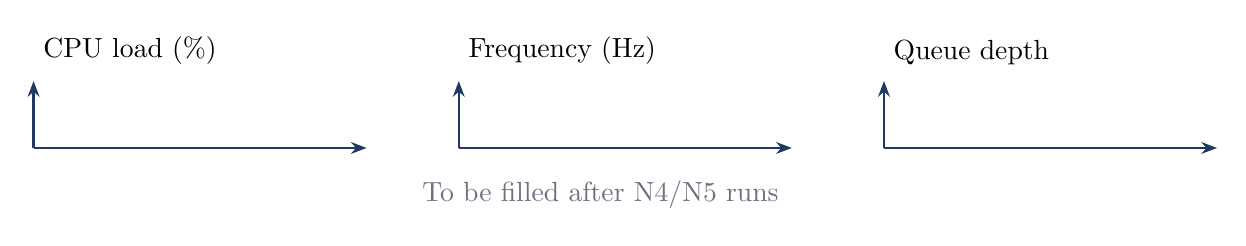
\begin{tikzpicture}[x=.90cm,y=.85cm,font=\normalsize,box/.append style={font=\normalsize}]
\foreach \x/\lab in {0/CPU load (\%),6/Frequency (Hz),12/Queue depth}{\draw[flow] (\x,0)--(\x+4.7,0);\draw[flow] (\x,0)--(\x,1.0);\node[anchor=south west] at (\x,1.1){\lab};}
\node[text=muted] at (8,-.7){To be filled after N4/N5 runs};
\end{tikzpicture}}{Summaries have evidence; missing joined time-series panels stay empty.}\par\vfill\takeaway{Stable power is required before interpreting processor performance. (Figure~\ref{fig:D78})}\note{Evidence: experiments/2026-10-13-n4a-euroc-mh01/REPORT.md. Deck authoring only; no camera, Pi or ORB program was executed in Phase 6.}\end{frame}
\begin{frame}{6.1 Runtime and USB}\evidence{PLANNED}
\deckitems{\item Default: native Pi baseline and direct known-good USB3 cable.\item Docker adds package, device and user/group boundaries.\item A hub/storage topology can change shared power and bandwidth.\item Revisit only after equivalent physical gates and clear deployment benefit.}
\vfill
\begin{tabular}{L{87.0mm}L{87.0mm}}\toprule
\textbf{Default} & \textbf{Evidence that changes it}\\\midrule
Native Pi & Equivalent gates + packaging benefit\\[5pt]
Direct USB3 & Alternative topology sustains speed/power/load\\[5pt]
\bottomrule\end{tabular}
\vfill\takeaway{Packaging cannot compensate for a 480M camera branch.}
\note{Container portability is useful only after identical sensor, clock and recording evidence. Connector shape is not negotiated speed. Shared-storage trials need own-branch speed, power and sustained-load evidence. Source register: N,H,G. Recommend native Pi/direct known-good USB-A↔USB-C; containers/topology changes need equivalent qualification and reproducibility benefit.}\end{frame}
\begin{frame}{6.2 Inputs and clocks}\evidence{PLANNED}
\deckitems{\item Keep exact IR1 640$\times$480/15 qualification unchanged.\item Stereo starts with matching profiles as a reviewed extension.\item Emitter-off is a separate natural-feature tracking experiment.\item Preserve global-time readback and original timestamp domains.}
\vfill
\begin{tabular}{L{87.0mm}L{87.0mm}}\toprule
\textbf{Default} & \textbf{Evidence that changes it}\\\midrule
Exact baseline profiles & Paired quality / tail-load comparison\\[5pt]
Preserved emitter state & Separate controlled natural-feature trial\\[5pt]
Logged global-time state & Measured domains/drift/offset evidence\\[5pt]
\bottomrule\end{tabular}
\vfill\takeaway{Change one input variable with paired quality and load evidence.}
\note{More resolution/rate may improve features but increases blur, bandwidth or CPU trade-offs. Preserve accepted emitter setting; compare off/on under controlled scene/lighting. Global time off/on diagnostics require separate evidence; no silent stamp rewrite or assumed zero offset. Source register: G,C,U. Keep accepted IR1 640$\times$480/15 gate; PLANNED stereo starts there; emitter-off feature trials are separate; global time needs domain evidence.}\end{frame}
\begin{frame}{6.3 Algorithm and calibration}\evidence{PLANNED}
\deckitems{\item Validate upstream EuRoC and offline inputs before live wrapper.\item Candidate: Kalibr spatial/time calibration plus measured IMU noise.\item Choose tools from import/build/model compatibility and residuals.\item Defer wheel odometry until timing, frames and slip evidence exist.}
\vfill
\begin{tabular}{L{87.0mm}L{87.0mm}}\toprule
\textbf{Default} & \textbf{Evidence that changes it}\\\midrule
Upstream then offline & Matched-data wrapper equivalence\\[5pt]
Measured calibration/noise & Tool compatibility + holdout residuals\\[5pt]
Defer wheel fusion & Synchronized geometry + slip evidence\\[5pt]
\bottomrule\end{tabular}
\par\medskip\textbf{Tool qualification}: Kalibr spatial/time calibration and imu\_utils noise analysis are candidates. Test bag import, models and holdout residuals.\par\vfill\takeaway{Add complexity only to solve a measured failure mode.}
\note{A ROS wrapper helps integration but adds queues, pairing and revision differences. Matched-data comparison should establish behavior before choosing the path. Wheel fusion needs synchronized encoders, geometry and slip handling; no fusion node is designed here. Source register: A,O,C,B. Upstream EuRoC/offline before wrapper/live; Kalibr candidate plus measured noise; wheel odometry waits for timing/frame/slip evidence.}\note{Merged original page 40: 
\deckitems{\item Kalibr is a candidate for camera–IMU geometry and time offset. \hyperlink{referencepage}{[6]} \item imu\_utils is a candidate for stationary noise analysis.\item Bag import, camera model and dependency compatibility need tests.\item Select tools using residuals, holdout data and reproducibility.}
\vfill
\begin{tabular}{L{87.0mm}L{87.0mm}}\toprule
\textbf{Candidate} & \textbf{Role / remaining constraint}\\\midrule
Kalibr & Spatial/time estimation; import/model/build\\[5pt]
imu\_utils & Noise analysis; precision/duration/build\\[5pt]
Holdout checks & Residuals, repeatability and provenance\\[5pt]
\bottomrule\end{tabular}
\vfill\takeaway{A tool name is not a calibration plan or accepted result.}
Kalibr ROS1-oriented bag support does not imply direct ROS2 bag acceptance. Preserve originals and review an import/conversion path. imu\_utils does not supply complete stereo/camera–IMU calibration. No dependency install or format implementation is authorized. Source register: K,I,C. PLANNED Kalibr handles spatial/temporal estimation; imu\_utils handles noise, not complete calibration; import/build trade-offs remain.}\end{frame}
\begin{frame}{7.1 Historical evidence}\evidence{HISTORICAL / MEASURED saved observations}
\deckitems{\item 8 September: x86 virtual machine (VM)/Docker USB2 NO-GO. (Figure~\ref{fig:D85})\item 12/13 September: Pi saw 5000M, then USB regressed to 480M.\item A historical 105-second capture did not complete N2.\item Archived optimistic PASS wording cannot promote current gates.}
\vfill
\coursefigure{D85}{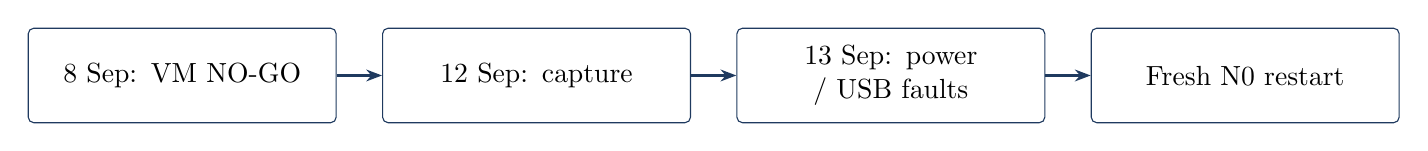
\begin{tikzpicture}[y=.70cm]
\node[box,font=\normalsize,text width=37.0mm,minimum height=12mm] (a0) at (0.0,0) {8 Sep: VM NO-GO};
\node[box,font=\normalsize,text width=37.0mm,minimum height=12mm] (a1) at (4.5,0) {12 Sep: capture};
\draw[flow] (a0.east) -- (a1.west);
\node[box,font=\normalsize,text width=37.0mm,minimum height=12mm] (a2) at (9.0,0) {13 Sep: power / USB faults};
\draw[flow] (a1.east) -- (a2.west);
\node[box,font=\normalsize,text width=37.0mm,minimum height=12mm] (a3) at (13.5,0) {Fresh N0 restart};
\draw[flow] (a2.east) -- (a3.west);\end{tikzpicture}}{Historical evidence; schematic.}
\vfill\takeaway{History explains risks; restart acceptance from fresh N0.}
\note{Sources: baseline audit, Pi-native validation report, evidence reconciliation and calibration readiness. Historical raw CSV/PGM files from the 105-second capture are absent from this Mac repository. Retain saved analyses/logs and the limitation. Source register: H,E,B. September 8 x86 VM/Docker NO-GO; September 12/13 history cannot promote current gates; 105-second run was not final N2.}\end{frame}
\begin{frame}{7.2 Current evidence gaps}\evidence{MEASURED progress / qualification OPEN}
\par\begin{tabular}{@{}L{72mm}L{112mm}@{}}\toprule\textbf{Layer} & \textbf{Current status on 13 October}\\\midrule
N0--N3: platform / new unit & OPEN; under-voltage and storage qualification unresolved\\[6pt]N4A: EuRoC MH01 & MEASURED accuracy; OPEN for power rerun / contract review\\[6pt]N4B / N4C: D435i & Programs BUILT, never run; calibration unqualified\\[6pt]N5--N7: metrics / health / STM32 & Partial N4A metrics only; campaign and integration PLANNED\\[6pt]\bottomrule\end{tabular}\par\vfill\takeaway{No Pi gate has passed; measured progress and qualification gaps coexist.}\note{Evidence: experiments/2026-10-13-SESSION\_FACTS\_FOR\_SLIDES.md; experiments/2026-10-13-n4a-euroc-mh01/REPORT.md. Deck authoring only; no camera, Pi or ORB program was executed in Phase 6.}\end{frame}
\begin{frame}{7.3 Changes since 2026-10-10}\evidence{MEASURED progress / no gate PASS}
\par\begin{tabular}{@{}L{77mm}L{107mm}@{}}\toprule\textbf{Change} & \textbf{Meaning / remaining limit}\\\midrule
4 GB Pi / 32 GB microSD stand-in & 8 GB / qualified bulk storage remains target; unstable power\\[6pt]New D435i: SDK 317422076650 & USB/ASIC 327743061057; old receipts do not transfer\\[6pt]Three EuRoC MH01 runs & ATE 0.0415 / 0.0368 / 0.0416 m; N4A OPEN\\[6pt]Recorder + D435i estimator built & Offline/live camera modes never run; calibration unqualified\\[6pt]\bottomrule\end{tabular}\par\medskip B explains the build, programs and next actions; C retains their gate contracts.\vfill\takeaway{Repair power; refresh N0 before new-unit N1, N2 and N3.}\note{Evidence: experiments/2026-10-13-SESSION\_FACTS\_FOR\_SLIDES.md; experiments/2026-10-13-n4a-euroc-mh01/REPORT.md. Deck authoring only; no camera, Pi or ORB program was executed in Phase 6.}\end{frame}
\begin{frame}{7.4 Conditional roadmap}\evidence{PLANNED}
\begin{columns}[T,onlytextwidth]\begin{column}{.48\textwidth}\deckitems{\item Repair supply; refresh camera-free N0 evidence. (Figure~\ref{fig:P12})\item After CAMERA AVAILABLE: N1 $\rightarrow$ N2 $\rightarrow$ N3.\item Rerun N4A with stable power; qualify stereo/calibration for N4B/C.\item Review N6; separately authorize N7.}\end{column}\begin{column}{.48\textwidth}
\coursefigure{P12}{\slideimg[.49\textheight]{\linewidth}{P12}{Conditional evidence journey}}{Conditional evidence journey; conceptual.}\end{column}\end{columns}
\vfill\takeaway{Advance on evidence, not dates or a successful launch.}
\note{The roadmap is conditional. Earlier transport gates block physical acquisition; independent algorithm planning remains useful but no ORB execution is authorized now. Preserve every failure and ask for the missing decision only when concrete evidence is ready. Source register: B,O,G. Fresh N0$\rightarrow$N1$\rightarrow$N2$\rightarrow$N3, reviewed stereo/calibration extension, N4A/B/C$\rightarrow$N5$\rightarrow$N6$\rightarrow$N7; blockers yield records, not deadline promises.}\end{frame}
\begin{frame}{8. Conclusion}\evidence{KNOWN ownership / PLANNED qualification}
\deckitems{\item Trusted perception needs qualified input, clocks and calibration.\item Repeated estimation and explicit metrics support engineering decisions.\item Independent controller ownership limits perception failure propagation.\item Status: N4A accuracy measured; no Pi gate passed; repair power next.}
\vfill
\begin{block}{Engineering decision}The owner gains a bounded sequence for directing agents and interpreting evidence.\end{block}
\vfill\takeaway{The guide supplies a reproducible path, not measured robot readiness.}
\note{Contribution: one source-grounded gate ladder, ownership boundary, implementation/data/clock model, evaluation contract and bounded AI tickets. The owner can direct agents without conflating tooling tests and hardware evidence. Physical balance and performance remain unverified. Source register: A,B,G. Trust needs qualified acquisition/timing/calibration/repeated estimation; controller independence protects balance; next step is N0 evidence.}\end{frame}
\begin{frame}{References}\hypertarget{referencepage}{}\footnotesize\begin{columns}[T,onlytextwidth]
\begin{column}{.48\textwidth}
\par\medskip\textbf{[1]} Campos, Elvira, Gómez Rodríguez, Montiel, Tardós. ORB-SLAM3. arXiv:2007.11898v2, 2021. \href{https://arxiv.org/abs/2007.11898}{Primary source}.
\par\medskip\textbf{[2]} Burri et al. The EuRoC micro aerial vehicle datasets. International Journal of Robotics Research, 2016. \href{https://projects.asl.ethz.ch/datasets/euroc-mav/}{Primary source}.
\par\medskip\textbf{[3]} ROS 2 Jazzy: Quality of Service documentation. \href{https://docs.ros.org/en/jazzy/Concepts/Intermediate/About-Quality-of-Service-Settings.html}{Primary source}.
\par\medskip\textbf{[4]} ROS REP-103 / REP-105: units, coordinates and frames. \href{https://www.ros.org/reps/rep-0105.html}{Primary source}.
\par\medskip\textbf{[5]} RealSense librealsense v2.58.4: timestamp reader and calibration parser. \href{https://github.com/realsenseai/librealsense/tree/v2.58.4}{Primary source}.
\end{column}
\begin{column}{.48\textwidth}
\par\medskip\textbf{[6]} ETH Zürich ASL: Kalibr camera–IMU calibration. \href{https://github.com/ethz-asl/kalibr/wiki/camera-imu-calibration}{Primary source}.
\par\medskip\textbf{[7]} gaowenliang: imu\_utils maintainer documentation. \href{https://github.com/gaowenliang/imu_utils}{Primary source}.
\par\medskip\textbf{[8]} Michael Grupp: evo trajectory metrics. \href{https://github.com/MichaelGrupp/evo/wiki/Metrics}{Primary source}.
\par\medskip\textbf{[9]} Raspberry Pi 5 / Active Cooler and RealSense D435i vendor records. \href{https://www.raspberrypi.com/products/raspberry-pi-5/}{Primary source}. \href{https://www.intel.com/content/www/us/en/products/sku/190004/intel-realsense-depth-camera-d435i/specifications.html}{D435i record}.
\end{column}
\end{columns}\vfill\normalsize N4A accuracy is measured; D435i and robot qualification remain OPEN.\end{frame}\end{document}
